\documentclass[11pt, a4paper, english]{article}\usepackage[]{graphicx}\usepackage[dvipsnames]{xcolor}
% maxwidth is the original width if it is less than linewidth
% otherwise use linewidth (to make sure the graphics do not exceed the margin)
\makeatletter
\def\maxwidth{ %
  \ifdim\Gin@nat@width>\linewidth
    \linewidth
  \else
    \Gin@nat@width
  \fi
}
\makeatother

\definecolor{fgcolor}{rgb}{0.345, 0.345, 0.345}
\newcommand{\hlnum}[1]{\textcolor[rgb]{0.686,0.059,0.569}{#1}}%
\newcommand{\hlstr}[1]{\textcolor[rgb]{0.192,0.494,0.8}{#1}}%
\newcommand{\hlcom}[1]{\textcolor[rgb]{0.678,0.584,0.686}{\textit{#1}}}%
\newcommand{\hlopt}[1]{\textcolor[rgb]{0,0,0}{#1}}%
\newcommand{\hlstd}[1]{\textcolor[rgb]{0.345,0.345,0.345}{#1}}%
\newcommand{\hlkwa}[1]{\textcolor[rgb]{0.161,0.373,0.58}{\textbf{#1}}}%
\newcommand{\hlkwb}[1]{\textcolor[rgb]{0.69,0.353,0.396}{#1}}%
\newcommand{\hlkwc}[1]{\textcolor[rgb]{0.333,0.667,0.333}{#1}}%
\newcommand{\hlkwd}[1]{\textcolor[rgb]{0.737,0.353,0.396}{\textbf{#1}}}%
\let\hlipl\hlkwb

\usepackage{framed}
\makeatletter
\newenvironment{kframe}{%
 \def\at@end@of@kframe{}%
 \ifinner\ifhmode%
  \def\at@end@of@kframe{\end{minipage}}%
  \begin{minipage}{\columnwidth}%
 \fi\fi%
 \def\FrameCommand##1{\hskip\@totalleftmargin \hskip-\fboxsep
 \colorbox{shadecolor}{##1}\hskip-\fboxsep
     % There is no \\@totalrightmargin, so:
     \hskip-\linewidth \hskip-\@totalleftmargin \hskip\columnwidth}%
 \MakeFramed {\advance\hsize-\width
   \@totalleftmargin\z@ \linewidth\hsize
   \@setminipage}}%
 {\par\unskip\endMakeFramed%
 \at@end@of@kframe}
\makeatother

\definecolor{shadecolor}{rgb}{.97, .97, .97}
\definecolor{messagecolor}{rgb}{0, 0, 0}
\definecolor{warningcolor}{rgb}{1, 0, 1}
\definecolor{errorcolor}{rgb}{1, 0, 0}
\newenvironment{knitrout}{}{} % an empty environment to be redefined in TeX

\usepackage{alltt}
%typesetting
\usepackage[margin = 1in]{geometry} % margins
\usepackage[T1]{fontenc} % font encoding
\usepackage{babel} %enables typesetting for multiple languages
\usepackage{parskip} %new lines
\usepackage{graphicx} 
\usepackage{float}
\floatplacement{figure}{H} %when printing tables, include  table.position="H"
\usepackage{bm}
\usepackage{amsmath}

\usepackage[dvipsnames]{xcolor} % more colors

\usepackage[colorlinks]{hyperref}


 %clickable table of contents from hyperref
\hypersetup{
    colorlinks,
    citecolor=black,
    filecolor=black,
    linkcolor=black,
    urlcolor=black
}

\usepackage[colorinlistoftodos]{todonotes}
\setcounter{secnumdepth}{0}

\title{Machine Learning 2ST129 26605 HT2023
 Assignment 1 }
\author{Anonymous Student}
\date{\today}
\IfFileExists{upquote.sty}{\usepackage{upquote}}{}
\begin{document}
\maketitle
\newpage
\tableofcontents
\newpage




\section{General Information}
\begin{itemize}
\item Time used for reading: about 6 hours
\item Time used for basic assignment: 18 hours
\item Time used for extra assignment 4 hours
\item Good with lab: Very practical. Now i know how to compute gradient descents.
\item Things to improve in the lab: Perhaps either more specified reading instructions or less reading. For example, i did not feel that everything in the articles was relevant and I just skipped most of it. Likewise with some of the pages in the book that were mandatory. 

I also started with the assignment the previous week, which made me do many tasks not included in this. Which is my own fault but just cost me some extra hours. Anyway, in case some of the tasks are still referenced wrong then it is probably because of that. 
\end{itemize}
\newpage




\section{Task 1: Basic, Stochastic, and Mini-Batch Gradient Descent}
\subsection{Gradient for logistic regression}
\subsubsection{Derive gradient}
For this task we want to derive the gradient for $NNL(\theta, \bm{y}, \bm{X}) = -l(\theta, \bm{y}, \bm{X})$ 
where we have that the likelihood function can be expressed as:
$$L(\theta, \bm{y}, \bm{X}) = \prod_{i=1}^n p_i^{y_i}(1-p_i)^{1-yi}$$

and the log likelihood:
\begin{align}
l(\theta, \mathbf{y}, \mathbf{X}) & =\sum_{i=1}^n y_i \log \left(p_i\right)+\left(1-y_i\right) \log \left(1-p_i\right) \\
& =\sum_{i=1}^n y_i \mathbf{x}_i \theta+\log \left(1-p_i\right) \\
& =\sum_{i=1}^n y_i \mathbf{x}_i \theta-\log \left(1+\exp \left(\mathbf{x}_i \theta\right)\right) .
\end{align}

%The gradient represents the vector of partial derivatives of the log likelihood with respect to each element of $\theta$:
%\begin{equation}
%\nabla L(f(x ; \theta), y)=\left[\begin{array}{c}
%\frac{\partial}{\partial w_1} L(f(x ; \theta), y) \\
%\frac{\partial}{\partial w_2} L(f(x ; \theta), y) \\
%\vdots \\
%\frac{\partial}{\partial w_n} L(f(x ; \theta), y) \\
%\frac{\partial}{\partial b} L(f(x ; \theta), y)
%\end{array}\right]
%\end{equation}

The partial derivatives of the log likelihood with respect to the different parameters can be expressed as:
\[
\frac{\partial l}{\partial \theta_j} = \sum_{i=1}^n \left(y_i x_{ij} - \frac{x_{ij} \exp(\mathbf{x}_i \theta)}{1 + \exp(\mathbf{x}_i \theta)}\right)
\]

Then we have that the gradient is simply when we take the partial derivatives of the log-likelihood function with respect to all parameters such that:


\[
\nabla l(\theta, \mathbf{y}, \mathbf{X}) =-  \left(\frac{\partial l}{\partial \theta_1}, \frac{\partial l}{\partial \theta_2}, \ldots, \frac{\partial l}{\partial \theta_p}\right)
\]

Where \(p\) is the number of parameters in the vector \(\theta\).
If we instead write it in matrix form, then it can be expressed as:
\[\nabla l(\theta, \mathbf{y}, \mathbf{X}) = - \mathbf{X}^T (\mathbf{y} - \mathbf{p}) \]

where we have that
$\bm{y}$ is a vector of the values of $y_i$.
$\bm{X}$is the $ N \times (p+1) $ design matrix of $x_i$ values, $\bm{P}$  is the vector of fitted probabilities $p_i$

It is this matrix notation we will work with in practise when we compute the gradient in R.
\subsubsection{Implement gradient in R}


\begin{knitrout}
\definecolor{shadecolor}{rgb}{0.969, 0.969, 0.969}\color{fgcolor}\begin{kframe}
\begin{alltt}
\hlcom{#Libraries}
 \hlkwd{library}\hlstd{(tidyverse)}
 \hlkwd{library}\hlstd{(xtable)}
 \hlkwd{library}\hlstd{(uuml)}
 \hlkwd{library}\hlstd{(gridExtra)}
 \hlkwd{library}\hlstd{(glmnet)}
 \hlkwd{library}\hlstd{(parallel)}
\end{alltt}
\end{kframe}
\end{knitrout}


\begin{knitrout}
\definecolor{shadecolor}{rgb}{0.969, 0.969, 0.969}\color{fgcolor}\begin{kframe}
\begin{alltt}
\hlkwd{data}\hlstd{(}\hlstr{"binary"}\hlstd{)}
\hlstd{binary}\hlopt{$}\hlstd{gre_sd} \hlkwb{<-} \hlstd{(binary}\hlopt{$}\hlstd{gre} \hlopt{-} \hlkwd{mean}\hlstd{(binary}\hlopt{$}\hlstd{gre))} \hlopt{/}\hlkwd{sd}\hlstd{(binary}\hlopt{$}\hlstd{gre)}
\hlstd{binary}\hlopt{$}\hlstd{gpa_sd} \hlkwb{<-} \hlstd{(binary}\hlopt{$}\hlstd{gpa} \hlopt{-} \hlkwd{mean}\hlstd{(binary}\hlopt{$}\hlstd{gpa))} \hlopt{/}\hlkwd{sd}\hlstd{(binary}\hlopt{$}\hlstd{gpa)}
\hlstd{X} \hlkwb{<-} \hlkwd{model.matrix}\hlstd{(admit} \hlopt{~} \hlstd{gre_sd} \hlopt{+} \hlstd{gpa_sd, binary)}
\hlstd{y} \hlkwb{<-} \hlstd{binary}\hlopt{$}\hlstd{admit}
\end{alltt}
\end{kframe}
\end{knitrout}


\begin{knitrout}
\definecolor{shadecolor}{rgb}{0.969, 0.969, 0.969}\color{fgcolor}\begin{kframe}
\begin{alltt}
\hlcom{#' gradient function}
\hlcom{#' @param y  vector of observations outcomes}
\hlcom{#' @param X Data Matrix}
\hlcom{#' @param theta Parameters}
\hlcom{#' @return The gradient}

\hlcom{# Gradient function}
\hlstd{ll_grad} \hlkwb{<-} \hlkwa{function}\hlstd{(}\hlkwc{y}\hlstd{,} \hlkwc{X}\hlstd{,} \hlkwc{theta}\hlstd{) \{}
  \hlstd{n} \hlkwb{<-} \hlkwd{length}\hlstd{(y)}
  \hlstd{P} \hlkwb{<-} \hlnum{1} \hlopt{/} \hlstd{(}\hlnum{1} \hlopt{+} \hlkwd{exp}\hlstd{(}\hlopt{-}\hlstd{X} \hlopt \hlstd{theta))}
  \hlstd{grad} \hlkwb{<-} \hlkwd{t}\hlstd{(X)} \hlopt \hlstd{(y}\hlopt{-}\hlstd{P)} \hlopt{/} \hlstd{n}
  \hlkwd{return}\hlstd{(grad)}
\hlstd{\}}


\hlkwd{round}\hlstd{(}\hlkwd{t}\hlstd{(}\hlkwd{ll_grad}\hlstd{(y, X,} \hlkwc{theta} \hlstd{=} \hlkwd{c}\hlstd{(}\hlnum{0}\hlstd{,} \hlnum{0}\hlstd{,} \hlnum{0}\hlstd{))),} \hlnum{4}\hlstd{)}
\end{alltt}
\begin{verbatim}
     (Intercept) gre_sd gpa_sd
[1,]     -0.1825 0.0857 0.0829
\end{verbatim}
\begin{alltt}
\hlkwd{round}\hlstd{(}\hlkwd{t}\hlstd{(}\hlkwd{ll_grad}\hlstd{(y, X,} \hlkwc{theta} \hlstd{=} \hlkwd{c}\hlstd{(}\hlopt{-}\hlnum{1}\hlstd{,} \hlnum{0.5}\hlstd{,} \hlnum{0.5}\hlstd{))),} \hlnum{4}\hlstd{)}
\end{alltt}
\begin{verbatim}
     (Intercept)  gre_sd  gpa_sd
[1,]      0.0217 -0.0395 -0.0426
\end{verbatim}
\end{kframe}
\end{knitrout}
\subsection{Implement Gradient Descent}
\subsubsection{1}
Here we just print the values from the fitted logistic regression:

\begin{knitrout}
\definecolor{shadecolor}{rgb}{0.969, 0.969, 0.969}\color{fgcolor}\begin{kframe}
\begin{alltt}
\hlstd{theta} \hlkwb{<-} \hlkwd{c}\hlstd{(}\hlnum{0}\hlstd{,} \hlnum{0}\hlstd{,} \hlnum{0}\hlstd{)}
\hlkwd{ll}\hlstd{(y, X, theta)}
\end{alltt}
\begin{verbatim}
[1] -277.2589
\end{verbatim}
\begin{alltt}
\hlkwd{glm}\hlstd{(y} \hlopt{~}\hlstd{X}  \hlopt{-}\hlnum{1} \hlstd{,} \hlkwc{family} \hlstd{=} \hlkwd{binomial}\hlstd{(}\hlkwc{link} \hlstd{=} \hlstr{"logit"}\hlstd{))}\hlopt{$}\hlstd{coefficients} \hlopt
  \hlkwd{print}\hlstd{()}
\end{alltt}
\begin{verbatim}
X(Intercept)      Xgre_sd      Xgpa_sd 
  -0.8097503    0.3108184    0.2872087 
\end{verbatim}
\end{kframe}
\end{knitrout}

\subsubsection{2}

Now we want to implement the different gradient descent algorithms.
\begin{knitrout}
\definecolor{shadecolor}{rgb}{0.969, 0.969, 0.969}\color{fgcolor}\begin{kframe}
\begin{alltt}
\hlcom{#' Batch gradient descent}
\hlcom{#' @param  learn_rate the step size}
\hlcom{#' @param epochs number of iterations}

\hlstd{batch_gsd} \hlkwb{<-} \hlkwa{function}\hlstd{(}\hlkwc{y}\hlstd{,} \hlkwc{X}\hlstd{,} \hlkwc{theta} \hlstd{=} \hlkwd{rep}\hlstd{(}\hlnum{0}\hlstd{,} \hlkwd{ncol}\hlstd{(X)),} \hlkwc{learn_rate}\hlstd{,} \hlkwc{epochs}\hlstd{) \{}
    \hlstd{results} \hlkwb{<-} \hlkwd{matrix}\hlstd{(}\hlnum{0.0}\hlstd{,} \hlkwc{ncol} \hlstd{=} \hlkwd{ncol}\hlstd{(X)} \hlopt{+} \hlnum{2L}\hlstd{,} \hlkwc{nrow} \hlstd{= epochs)}
  \hlkwd{colnames}\hlstd{(results)} \hlkwb{<-} \hlkwd{c}\hlstd{(}\hlstr{"epoch"}\hlstd{,} \hlstr{"nll"}\hlstd{,} \hlkwd{colnames}\hlstd{(X))}
  \hlkwa{for} \hlstd{(epoch} \hlkwa{in} \hlnum{1}\hlopt{:}\hlstd{epochs) \{}
    \hlstd{gradient} \hlkwb{<-} \hlopt{-}\hlkwd{ll_grad}\hlstd{(y, X, theta)} \hlcom{#negative gradient}
    \hlstd{theta} \hlkwb{<-} \hlstd{theta} \hlopt{-} \hlstd{(learn_rate} \hlopt{*} \hlstd{gradient)}

    \hlstd{results[epoch,} \hlstr{"epoch"}\hlstd{]} \hlkwb{<-} \hlstd{epoch}
    \hlstd{results[epoch,} \hlstr{"nll"}\hlstd{]} \hlkwb{<-} \hlkwd{ll}\hlstd{(y, X, theta)}
    \hlstd{results[epoch,} \hlopt{-}\hlstd{(}\hlnum{1}\hlopt{:}\hlnum{2}\hlstd{)]} \hlkwb{<-} \hlstd{theta}
  \hlstd{\}}
  \hlkwd{attributes}\hlstd{(results)}\hlopt{$}\hlstd{learn_rate} \hlkwb{<-} \hlstd{learn_rate}
  \hlkwd{attributes}\hlstd{(results)}\hlopt{$}\hlstd{epochs} \hlkwb{<-} \hlstd{epochs}
  \hlkwd{return}\hlstd{(results)}
\hlstd{\}}
\end{alltt}
\end{kframe}
\end{knitrout}

\begin{knitrout}
\definecolor{shadecolor}{rgb}{0.969, 0.969, 0.969}\color{fgcolor}\begin{kframe}
\begin{alltt}
\hlstd{stochastic_gsd} \hlkwb{<-} \hlkwa{function}\hlstd{(}\hlkwc{y}\hlstd{,} \hlkwc{X}\hlstd{,} \hlkwc{theta} \hlstd{=} \hlkwd{rep}\hlstd{(}\hlnum{0}\hlstd{,} \hlkwd{ncol}\hlstd{(X)),}
                                   \hlkwc{learn_rate}\hlstd{,} \hlkwc{epochs}\hlstd{,} \hlkwc{seed}\hlstd{=}\hlnum{1337} \hlstd{)\{}
  \hlkwd{set.seed}\hlstd{(seed)}
  \hlstd{results} \hlkwb{<-} \hlkwd{matrix}\hlstd{(}\hlnum{0.0}\hlstd{,} \hlkwc{ncol} \hlstd{=} \hlkwd{ncol}\hlstd{(X)} \hlopt{+} \hlnum{2L}\hlstd{,} \hlkwc{nrow} \hlstd{= epochs)}
  \hlkwd{colnames}\hlstd{(results)} \hlkwb{<-} \hlkwd{c}\hlstd{(}\hlstr{"epoch"}\hlstd{,} \hlstr{"nll"}\hlstd{,} \hlkwd{colnames}\hlstd{(X))}
    \hlkwa{for} \hlstd{(epoch} \hlkwa{in} \hlnum{1}\hlopt{:}\hlstd{epochs) \{}
      \hlstd{index_order} \hlkwb{<-} \hlkwd{sample}\hlstd{(}\hlkwd{length}\hlstd{(y))}
      \hlcom{#shuffle the data by indexing in a random order}

      \hlkwa{for} \hlstd{(i} \hlkwa{in} \hlstd{index_order )\{}
    \hlstd{gradient} \hlkwb{<-} \hlopt{-}\hlkwd{ll_grad}\hlstd{(y[i], X[i,,} \hlkwc{drop}\hlstd{=}\hlnum{FALSE}\hlstd{], theta)}
    \hlcom{#dont drop "redundant" information to keep it as a matrix}
   \hlstd{theta} \hlkwb{<-} \hlstd{theta} \hlopt{-} \hlstd{(learn_rate} \hlopt{*} \hlstd{gradient)}
      \hlstd{\}}
    \hlstd{results[epoch,} \hlstr{"epoch"}\hlstd{]} \hlkwb{<-} \hlstd{epoch}
    \hlstd{results[epoch,} \hlstr{"nll"}\hlstd{]} \hlkwb{<-} \hlkwd{ll}\hlstd{(y, X, theta)}
    \hlstd{results[epoch,} \hlopt{-}\hlstd{(}\hlnum{1}\hlopt{:}\hlnum{2}\hlstd{)]} \hlkwb{<-} \hlstd{theta}

    \hlstd{\}}
  \hlkwd{attributes}\hlstd{(results)}\hlopt{$}\hlstd{learn_rate} \hlkwb{<-} \hlstd{learn_rate}
  \hlkwd{attributes}\hlstd{(results)}\hlopt{$}\hlstd{epochs} \hlkwb{<-} \hlstd{epochs}
  \hlkwd{return}\hlstd{(results)}
\hlstd{\}}
\end{alltt}
\end{kframe}
\end{knitrout}

\begin{knitrout}
\definecolor{shadecolor}{rgb}{0.969, 0.969, 0.969}\color{fgcolor}\begin{kframe}
\begin{alltt}
\hlstd{minibatch_gsd} \hlkwb{<-} \hlkwa{function}\hlstd{(}\hlkwc{y}\hlstd{,} \hlkwc{X}\hlstd{,} \hlkwc{theta} \hlstd{=} \hlkwd{rep}\hlstd{(}\hlnum{0}\hlstd{,} \hlkwd{ncol}\hlstd{(X)),}
                          \hlkwc{sample_size}\hlstd{,} \hlkwc{learn_rate}\hlstd{,} \hlkwc{epochs}\hlstd{,}
                          \hlkwc{batch_size}\hlstd{,} \hlkwc{seed}\hlstd{=}\hlnum{1337}\hlstd{)\{}
  \hlkwd{set.seed}\hlstd{(seed)}
  \hlstd{n} \hlkwb{<-} \hlkwd{length}\hlstd{(y)}
  \hlstd{num_batches} \hlkwb{<-} \hlkwd{ceiling}\hlstd{(n}\hlopt{/}\hlstd{batch_size)}

\hlstd{results} \hlkwb{<-} \hlkwd{matrix}\hlstd{(}\hlnum{0.0}\hlstd{,} \hlkwc{ncol} \hlstd{=} \hlkwd{ncol}\hlstd{(X)} \hlopt{+} \hlnum{2L}\hlstd{,} \hlkwc{nrow} \hlstd{= epochs)}
\hlkwd{colnames}\hlstd{(results)} \hlkwb{<-} \hlkwd{c}\hlstd{(}\hlstr{"epoch"}\hlstd{,} \hlstr{"nll"}\hlstd{,} \hlkwd{colnames}\hlstd{(X))}

\hlcom{# Run algorithm}
\hlkwa{for}\hlstd{(epoch} \hlkwa{in} \hlnum{1}\hlopt{:}\hlstd{epochs)\{}
 \hlstd{index_order} \hlkwb{<-} \hlkwd{sample}\hlstd{(}\hlkwd{length}\hlstd{(y))}
 \hlcom{#shuffle the data by indexing in a random order}

\hlcom{### Put the algorithm code here ### }
  \hlkwa{for} \hlstd{(i} \hlkwa{in} \hlnum{1}\hlopt{:}\hlstd{num_batches)\{}

     \hlstd{batch_index} \hlkwb{<-} \hlkwd{which}\hlstd{(}\hlkwd{findInterval}\hlstd{(index_order,}
                                       \hlkwd{seq}\hlstd{(}\hlnum{1}\hlstd{, n,} \hlkwc{by} \hlstd{= batch_size))} \hlopt{==} \hlstd{i)}
     \hlcom{#which x and y  to subset for each iteration by }
     \hlcom{#dividing indexes to different batches}
    \hlstd{batch_X} \hlkwb{<-} \hlstd{X[batch_index,]}
    \hlstd{batch_y} \hlkwb{<-} \hlstd{y[batch_index]}

    \hlstd{gradient} \hlkwb{<-} \hlopt{-}\hlkwd{ll_grad}\hlstd{(}\hlkwc{y}\hlstd{=batch_y,} \hlkwc{X} \hlstd{= batch_X,} \hlkwc{theta}\hlstd{=theta )} \hlopt{/} \hlstd{batch_size}
   \hlstd{theta} \hlkwb{<-} \hlstd{theta} \hlopt{-} \hlstd{(learn_rate} \hlopt{*} \hlstd{gradient)}
  \hlstd{\}}
 \hlcom{# Store epoch, nll and output results}
\hlstd{results[epoch,} \hlstr{"epoch"}\hlstd{]} \hlkwb{<-} \hlstd{epoch}
\hlstd{results[epoch,} \hlstr{"nll"}\hlstd{]} \hlkwb{<-} \hlkwd{ll}\hlstd{(y, X, theta)}
\hlstd{results[epoch,} \hlopt{-}\hlstd{(}\hlnum{1}\hlopt{:}\hlnum{2}\hlstd{)]} \hlkwb{<-} \hlstd{theta}
\hlstd{\}}

\hlkwd{attributes}\hlstd{(results)}\hlopt{$}\hlstd{learn_rate} \hlkwb{<-} \hlstd{learn_rate}
\hlkwd{attributes}\hlstd{(results)}\hlopt{$}\hlstd{epochs} \hlkwb{<-} \hlstd{epochs}
\hlkwd{return}\hlstd{(results)}
\hlstd{\}}
\end{alltt}
\end{kframe}
\end{knitrout}


\subsubsection{3}
Now we want to try different three different values of the learning parameter $\eta$ and run the algorithm for 500 epochs.
To keep the report clean from unnecessary code, most of the code used for this task will be in the appendix. But the way it is structures is so that I made a plot function given the results from one of the gradient descent functions, and then i made all the previous functions, including the plot functions more generalized to multiple values of $\eta$ and then put into a main function for this task. Hence only the use of the main function will be presented here. 







\begin{knitrout}
\definecolor{shadecolor}{rgb}{0.969, 0.969, 0.969}\color{fgcolor}\begin{kframe}
\begin{alltt}
\hlstd{plots} \hlkwb{<-} \hlkwd{Task_1.3_main}\hlstd{(}\hlkwc{y}\hlstd{=y,}\hlkwc{X}\hlstd{=X,} \hlkwc{learn_rates} \hlstd{=} \hlkwd{list}\hlstd{(}\hlkwd{c}\hlstd{(}\hlnum{0.03}\hlstd{,}\hlnum{1}\hlstd{,}\hlnum{50}\hlstd{),}
                                                 \hlkwd{c}\hlstd{(}\hlnum{0.0001}\hlstd{,} \hlnum{0.001}\hlstd{,} \hlnum{1}\hlstd{),}
                                                 \hlkwd{c}\hlstd{(}\hlnum{0.05}\hlstd{,}\hlnum{1}\hlstd{,}\hlnum{15}\hlstd{)),}
                     \hlkwc{n_epochs}\hlstd{=}\hlnum{500}\hlstd{,} \hlkwc{seed}\hlstd{=}\hlnum{1337}\hlstd{,}
                     \hlkwc{batch_size} \hlstd{=} \hlnum{25}\hlstd{,}
                     \hlkwc{variable_name} \hlstd{=} \hlstr{"gre_sd"}\hlstd{)}
\end{alltt}
\end{kframe}
\end{knitrout}


\begin{knitrout}
\definecolor{shadecolor}{rgb}{0.969, 0.969, 0.969}\color{fgcolor}\begin{kframe}
\begin{alltt}
\hlkwd{plot}\hlstd{(plots}\hlopt{$}\hlstd{batch_GD)}
\end{alltt}
\end{kframe}\begin{figure}
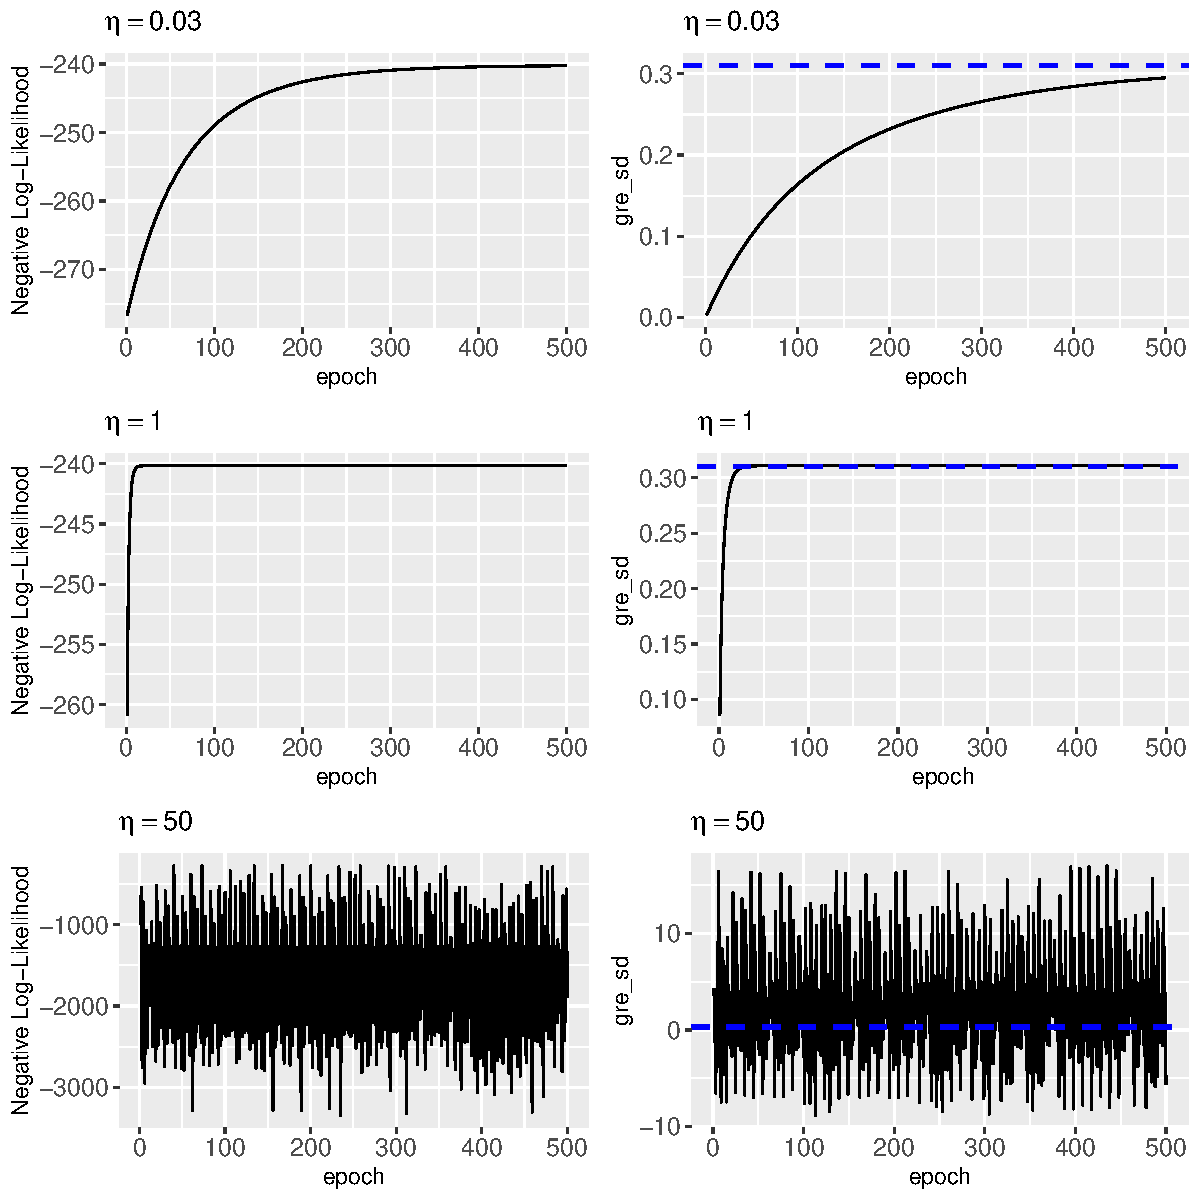
\includegraphics[width=\maxwidth]{figure/batch_results-1} \caption[Results for ordinary gradient descent]{Results for ordinary gradient descent}\label{fig:batch_results}
\end{figure}

\end{knitrout}

\begin{knitrout}
\definecolor{shadecolor}{rgb}{0.969, 0.969, 0.969}\color{fgcolor}\begin{kframe}
\begin{alltt}
\hlkwd{plot}\hlstd{(plots}\hlopt{$}\hlstd{stochastic_GD)}
\end{alltt}
\end{kframe}\begin{figure}
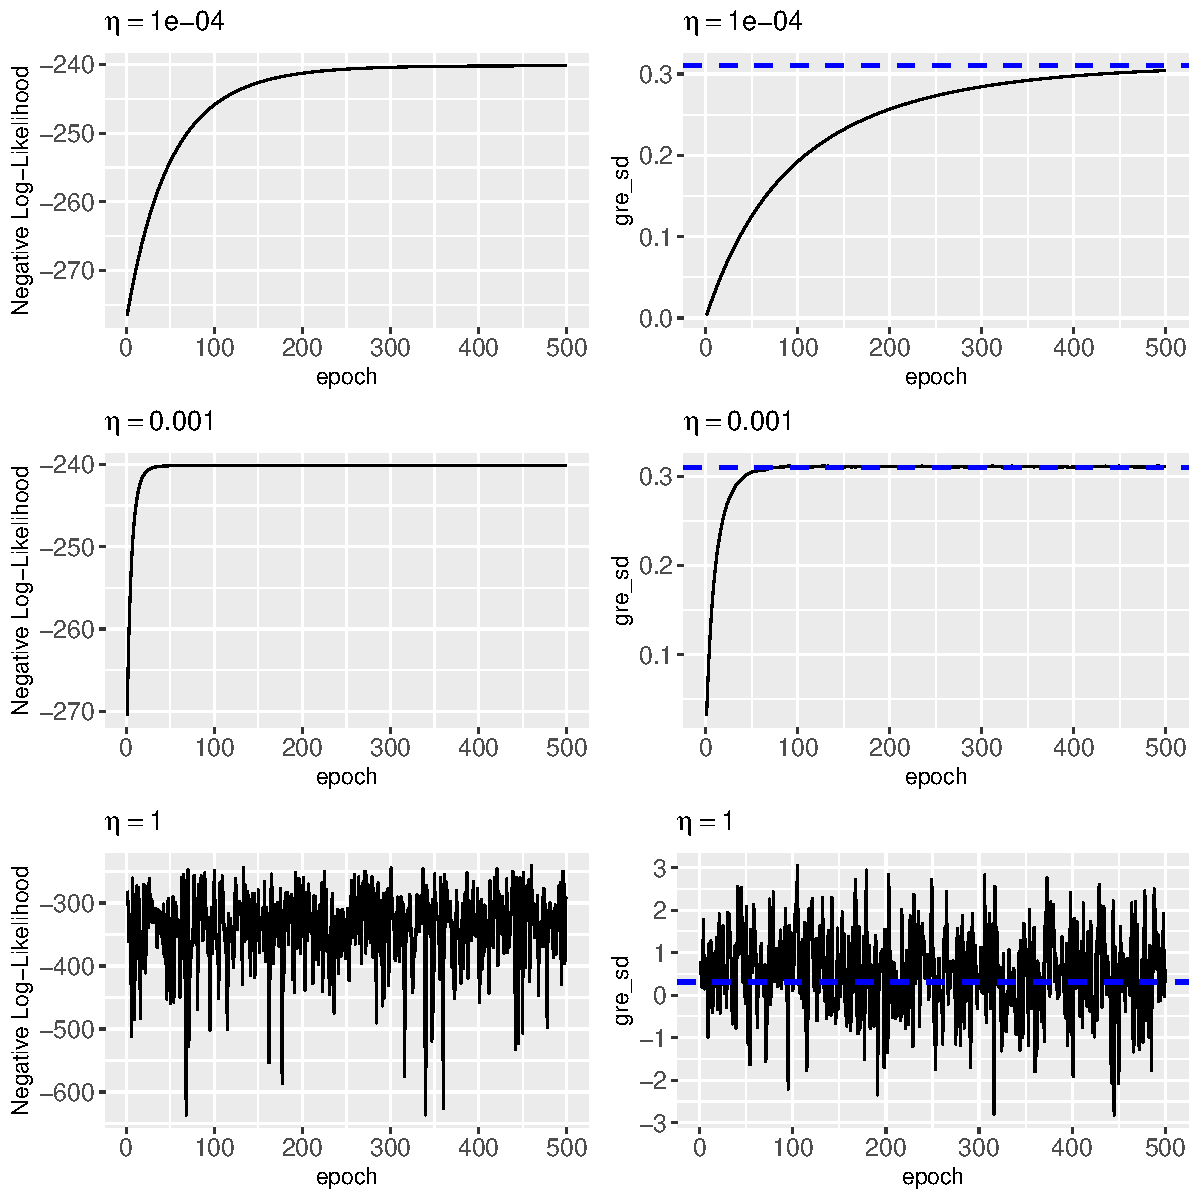
\includegraphics[width=\maxwidth]{figure/stochastic_results-1} \caption[Results for stochastic gradient descent]{Results for stochastic gradient descent}\label{fig:stochastic_results}
\end{figure}

\end{knitrout}

\begin{knitrout}
\definecolor{shadecolor}{rgb}{0.969, 0.969, 0.969}\color{fgcolor}\begin{kframe}
\begin{alltt}
\hlkwd{plot}\hlstd{(plots}\hlopt{$}\hlstd{minibatch_GD)}
\end{alltt}
\end{kframe}\begin{figure}
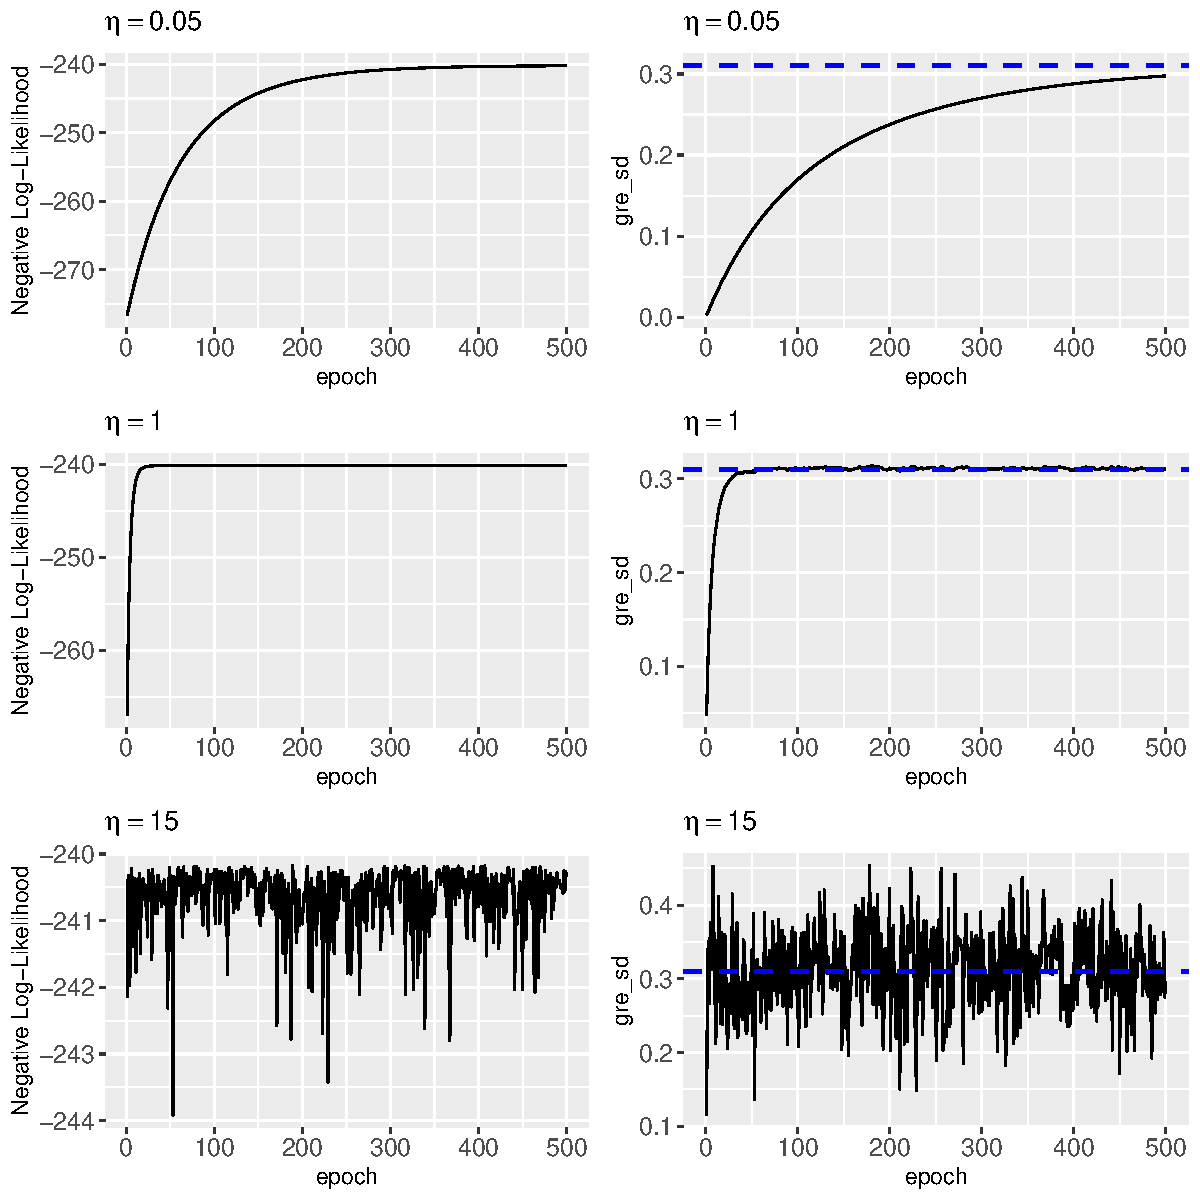
\includegraphics[width=\maxwidth]{figure/minibatch_results-1} \caption[Results for minibatch gradient descent]{Results for minibatch gradient descent}\label{fig:minibatch_results}
\end{figure}

\end{knitrout}




\section{Task 2: Regularized Regression}
\subsection{2.1 linear model}
Here we try to fit a linear model to the training data
\begin{knitrout}
\definecolor{shadecolor}{rgb}{0.969, 0.969, 0.969}\color{fgcolor}\begin{kframe}
\begin{alltt}
\hlstd{fit} \hlkwb{<-} \hlkwd{lm}\hlstd{( y} \hlopt{~} \hlstd{.,} \hlkwc{data}\hlstd{=prob2_train)}
\end{alltt}
\end{kframe}
\end{knitrout}
I wont show the full summary output due to there being many variables, but if we run the \texttt{summary()} function then we get some strange results. 
such as:
\begin{knitrout}
\definecolor{shadecolor}{rgb}{0.969, 0.969, 0.969}\color{fgcolor}\begin{kframe}
\begin{alltt}
Residuals:
ALL 200 residuals are 0: no residual degrees of freedom!

Residual standard error: NaN on 0 degrees of freedom
Multiple R-squared:      1,	Adjusted R-squared:    NaN 
F-statistic:   NaN on 199 and 0 DF,  p-value: NA
\end{alltt}
\end{kframe}
\end{knitrout}
as well as \texttt{Nan} for the std.error, t-values and p-values for the coefficients. This is most likely due to multicollinearity in the model, which is due to two or more variables are highly or perfectly correlated. This is perhaps not that surprising considering that there are 240 covariates. 

\subsection{2.2 Lasso regression}

Now we want to use the \texttt{glmnet()} function to fit a linear lasso regression with $\lambda$ = 1. 
Lasso is a regularization method which shrinks the coefficients by a penalty term $\lambda$ .
The  \texttt{glm.net()} works by fitting the penalized maximum likelihood glm-model with the specified elastic mixing parameter $\alpha$. If $\alpha=1$, which is the value we use in this case,  then its the the lasso penalty and if $\alpha = 0$ then it is the ridge penalty. 

\begin{knitrout}
\definecolor{shadecolor}{rgb}{0.969, 0.969, 0.969}\color{fgcolor}\begin{kframe}
\begin{alltt}
\hlstd{X} \hlkwb{<-} \hlkwd{as.matrix}\hlstd{(prob2_train[,} \hlopt{-}\hlnum{241}\hlstd{])}
\hlstd{y} \hlkwb{<-} \hlkwd{as.matrix}\hlstd{(prob2_train[,} \hlstr{"y"}\hlstd{])}
\hlstd{X_test} \hlkwb{<-} \hlkwd{as.matrix}\hlstd{(prob2_test[,} \hlopt{-}\hlnum{241}\hlstd{])}
\hlstd{y_test} \hlkwb{<-} \hlkwd{as.matrix}\hlstd{(prob2_test[,} \hlstr{"y"}\hlstd{])}
\hlstd{lasso_fit} \hlkwb{<-} \hlkwd{glmnet}\hlstd{(}\hlkwc{x}\hlstd{=X,} \hlkwc{y}\hlstd{=y,} \hlkwc{family} \hlstd{=} \hlstr{"gaussian"}\hlstd{,} \hlkwc{lambda}\hlstd{=}\hlnum{1}\hlstd{)}

\hlstd{lasso_coeffs} \hlkwb{<-} \hlkwd{coef}\hlstd{(lasso_fit)}
\end{alltt}
\end{kframe}
\end{knitrout}


The object \texttt{lasso\_coeffs} contains all the coefficients of the variables in a sparse format which are from the model corresponding to the lambda value. if we just look at the first and last values it looks like this:
\begin{knitrout}
\definecolor{shadecolor}{rgb}{0.969, 0.969, 0.969}\color{fgcolor}\begin{kframe}
\begin{alltt}
\hlkwd{head}\hlstd{(lasso_coeffs)}
\end{alltt}
\begin{verbatim}
6 x 1 sparse Matrix of class "dgCMatrix"
                   s0
(Intercept) 31.492961
V1           .       
V2           2.130597
V3           0.821336
V4           1.858161
V5           .       
\end{verbatim}
\begin{alltt}
\hlkwd{tail}\hlstd{(lasso_coeffs)}
\end{alltt}
\begin{verbatim}
6 x 1 sparse Matrix of class "dgCMatrix"
     s0
V235  .
V236  .
V237  .
V238  .
V239  .
V240  .
\end{verbatim}
\end{kframe}
\end{knitrout}
where the coefficients not used has a value of 0 represented by the dot. We can extract only the variables with non-zero values with this:
\begin{knitrout}
\definecolor{shadecolor}{rgb}{0.969, 0.969, 0.969}\color{fgcolor}\begin{kframe}
\begin{alltt}
\hlstd{used_coefs} \hlkwb{<-} \hlstd{lasso_coeffs[lasso_coeffs}\hlopt{@}\hlkwc{i}\hlopt{+}\hlnum{1}\hlstd{,]} \hlcom{#@ due to S4 class}
\hlkwd{print}\hlstd{(used_coefs)}
\end{alltt}
\begin{verbatim}
(Intercept)          V2          V3          V4          V6          V7 
 31.4929611   2.1305973   0.8213360   1.8581608  -5.2947105   0.8503707 
         V8          V9         V10 
  1.7790410   2.2202348   1.9040888 
\end{verbatim}
\begin{alltt}
\hlkwd{length}\hlstd{(used_coefs)}
\end{alltt}
\begin{verbatim}
[1] 9
\end{verbatim}
\end{kframe}
\end{knitrout}
Hence, only 8 variables were used for this model (intercept not included).

\subsection{2.3 - 2.4 10 fold cross validation}
Now we want to split the data into ten folds randomly  for task 2.3 and then implement a 10 fold cross-validation for task 2.4. I will just implement it in the same function here

The code for splitting the data into folds is this:
\begin{knitrout}
\definecolor{shadecolor}{rgb}{0.969, 0.969, 0.969}\color{fgcolor}\begin{kframe}
\begin{alltt}
\hlkwd{findInterval}\hlstd{(}\hlkwd{cut}\hlstd{(}\hlkwd{sample}\hlstd{(}\hlnum{1}\hlopt{:}\hlstd{n,n),}\hlkwc{breaks}\hlstd{=nfolds),}\hlnum{1}\hlopt{:}\hlstd{n)}
\end{alltt}
\end{kframe}
\end{knitrout}

which yields indexes ranging from 1 to the number of folds (10) for each observation.

I also define some helper functions to calculate the errors ( I originally made them when the questions were from the previous version of the assignment when you were supposed to have both MSE and RMSE, but after it changed I figured I might as well just keep the function as it is  and simply reuse it).
\begin{knitrout}
\definecolor{shadecolor}{rgb}{0.969, 0.969, 0.969}\color{fgcolor}\begin{kframe}
\begin{alltt}
\hlcom{#' function to calculate MSE and RMSE}
\hlstd{errors_func} \hlkwb{<-} \hlkwa{function}\hlstd{(}\hlkwc{y_obs}\hlstd{,} \hlkwc{pred}\hlstd{)\{}
  \hlstd{assertthat}\hlopt{::}\hlkwd{assert_that}\hlstd{(}\hlkwd{length}\hlstd{(y_obs)} \hlopt{==} \hlkwd{length}\hlstd{(pred),} \hlkwc{msg}\hlstd{=}\hlstr{"lengths differ"}\hlstd{)}
  \hlstd{n} \hlkwb{<-} \hlkwd{length}\hlstd{(y_obs)}
  \hlstd{Sum_square} \hlkwb{<-} \hlkwd{sum}\hlstd{( (y_obs} \hlopt{-} \hlstd{pred)}\hlopt{^}\hlnum{2}\hlstd{)}
  \hlstd{MSE} \hlkwb{<-} \hlstd{Sum_square} \hlopt{/} \hlstd{n}
  \hlstd{RMSE} \hlkwb{<-} \hlkwd{sqrt}\hlstd{(MSE)}
  \hlstd{res} \hlkwb{<-} \hlkwd{list}\hlstd{(}\hlstr{"MSE"}\hlstd{= MSE,} \hlstr{"RMSE"} \hlstd{= RMSE)}
  \hlkwd{return}\hlstd{(res)}
\hlstd{\}}
\end{alltt}
\end{kframe}
\end{knitrout}


\begin{knitrout}
\definecolor{shadecolor}{rgb}{0.969, 0.969, 0.969}\color{fgcolor}\begin{kframe}
\begin{alltt}
\hlstd{cross_validation} \hlkwb{<-} \hlkwa{function}\hlstd{(}\hlkwc{X}\hlstd{,} \hlkwc{y}\hlstd{,} \hlkwc{n_folds}\hlstd{,} \hlkwc{lambda}\hlstd{,} \hlkwc{alpha}\hlstd{=}\hlnum{1}\hlstd{,} \hlkwc{seed}\hlstd{=}\hlnum{1337}\hlstd{)\{}
  \hlstd{assertthat}\hlopt{::}\hlkwd{are_equal}\hlstd{(}\hlkwd{nrow}\hlstd{(X),}\hlkwd{length}\hlstd{(y),} \hlkwc{msg}\hlstd{=}\hlstr{"X and y dimension mismatch"}\hlstd{)}
  \hlstd{checkmate}\hlopt{::}\hlkwd{assert_int}\hlstd{(n_folds)}
  \hlkwd{set.seed}\hlstd{(seed)}

  \hlstd{n} \hlkwb{<-} \hlkwd{length}\hlstd{(y)}
  \hlstd{errors_matrix} \hlkwb{<-} \hlkwd{matrix}\hlstd{(}\hlnum{0}\hlstd{,} \hlkwc{nrow}\hlstd{= n_folds,} \hlkwc{ncol}\hlstd{=}\hlnum{2}\hlstd{)}
  \hlkwd{colnames}\hlstd{(errors_matrix)} \hlkwb{<-} \hlkwd{c}\hlstd{(}\hlstr{"MSE"}\hlstd{,} \hlstr{"RMSE"}\hlstd{)}

  \hlstd{Group}\hlkwb{=} \hlkwd{findInterval}\hlstd{(}\hlkwd{cut}\hlstd{(}\hlkwd{sample}\hlstd{(}\hlnum{1}\hlopt{:}\hlstd{n,n),}\hlkwc{breaks}\hlstd{=n_folds),}\hlnum{1}\hlopt{:}\hlstd{n)}
  \hlcom{#making n_folds equal groups.}
  \hlkwa{for} \hlstd{(i} \hlkwa{in} \hlnum{1}\hlopt{:}\hlstd{n_folds)\{}
  \hlstd{index} \hlkwb{<-} \hlkwd{which}\hlstd{(Group}\hlopt{==}\hlstd{i)}
  \hlcom{#index for which observations belongs to the current fold group}

  \hlstd{X_test} \hlkwb{<-} \hlstd{X[index,]}
  \hlstd{X_train} \hlkwb{<-} \hlstd{X[}\hlopt{-}\hlstd{index,]}
  \hlstd{y_test} \hlkwb{<-} \hlstd{y[index]}
  \hlstd{y_train} \hlkwb{<-} \hlstd{y[}\hlopt{-}\hlstd{index]}
  \hlstd{model} \hlkwb{<-}  \hlkwd{glmnet}\hlstd{(}\hlkwc{x}\hlstd{=X_train,} \hlkwc{y}\hlstd{=y_train,} \hlkwc{family} \hlstd{=} \hlstr{"gaussian"}\hlstd{,}
                     \hlkwc{lambda}\hlstd{=lambda,} \hlkwc{alpha}\hlstd{=alpha )}
  \hlstd{predictions} \hlkwb{<-} \hlkwd{predict}\hlstd{(model,} \hlkwc{s}\hlstd{=lambda,} \hlkwc{newx}\hlstd{=X_test,} \hlkwc{type}\hlstd{=}\hlstr{"response"}\hlstd{)}

  \hlstd{fold_errors} \hlkwb{<-} \hlkwd{errors_func}\hlstd{(}\hlkwc{y_obs} \hlstd{= y_test,} \hlkwc{pred}\hlstd{= predictions )}
  \hlstd{errors_matrix[i,}\hlnum{1}\hlstd{]} \hlkwb{<-} \hlstd{fold_errors}\hlopt{$}\hlstd{MSE}
  \hlstd{errors_matrix[i,}\hlnum{2}\hlstd{]} \hlkwb{<-} \hlstd{fold_errors}\hlopt{$}\hlstd{RMSE}


  \hlstd{\}}
  \hlstd{means} \hlkwb{<-} \hlkwd{apply}\hlstd{(errors_matrix,} \hlkwc{MARGIN}\hlstd{=}\hlnum{2}\hlstd{,} \hlkwc{FUN}\hlstd{=mean)}
  \hlkwd{return}\hlstd{(means)}
\hlstd{\}}
\end{alltt}
\end{kframe}
\end{knitrout}
Now that we have that function, to get the results for a single 10-fold validation with $\lambda=1$  we just use:
\begin{knitrout}
\definecolor{shadecolor}{rgb}{0.969, 0.969, 0.969}\color{fgcolor}\begin{kframe}
\begin{alltt}
\hlstd{results} \hlkwb{<-} \hlkwd{cross_validation}\hlstd{(}\hlkwc{X}\hlstd{= X,}\hlkwc{y}\hlstd{= y,} \hlkwc{n_folds}\hlstd{=}\hlnum{10}\hlstd{,} \hlkwc{lambda}\hlstd{=}\hlnum{1}\hlstd{)}
\hlkwd{print}\hlstd{(results)}
\end{alltt}
\begin{verbatim}
     MSE     RMSE 
9.986215 3.130366 
\end{verbatim}
\end{kframe}
\end{knitrout}
\subsection{2.5 5-fold cross-validation}
Now we just use the same function again but with \texttt{n\_folds=5} instead of 10.

\begin{knitrout}
\definecolor{shadecolor}{rgb}{0.969, 0.969, 0.969}\color{fgcolor}\begin{kframe}
\begin{alltt}
\hlstd{results2} \hlkwb{<-} \hlkwd{cross_validation}\hlstd{(}\hlkwc{X}\hlstd{= X,}\hlkwc{y}\hlstd{= y,} \hlkwc{n_folds}\hlstd{=}\hlnum{5}\hlstd{,} \hlkwc{lambda}\hlstd{=}\hlnum{1}\hlstd{)}
\hlkwd{print}\hlstd{(results2)}
\end{alltt}
\begin{verbatim}
      MSE      RMSE 
10.318704  3.172933 
\end{verbatim}
\end{kframe}
\end{knitrout}


Comparing the results for the 5-folds and the 10-folds, it is pretty close. However, the ten-fold cross-validation has slightly lower RMSE.
\section{2.6 different $\lambda$ }
Now to test different values of $\lambda$. 
Since the question is what is the best RMSE I can get, I will accept that challenge.  First I create a parallel version of the cross\_validation function to work for different $\lambda$-values. 

\begin{knitrout}
\definecolor{shadecolor}{rgb}{0.969, 0.969, 0.969}\color{fgcolor}\begin{kframe}
\begin{alltt}
\hlcom{#' @param export_vec vector of objects or functions to export to each cluster}

\hlstd{cross_validation_parallel} \hlkwb{<-} \hlkwa{function}\hlstd{(}\hlkwc{X}\hlstd{,} \hlkwc{y}\hlstd{,} \hlkwc{n_folds}\hlstd{,} \hlkwc{lambdas}\hlstd{,} \hlkwc{alpha}\hlstd{=}\hlnum{1}\hlstd{,} \hlkwc{seed}\hlstd{=}\hlnum{1337}\hlstd{,} \hlkwc{export_vec}\hlstd{)\{}
  \hlstd{n_cores} \hlkwb{<-} \hlstd{parallel}\hlopt{::}\hlkwd{detectCores}\hlstd{()}\hlopt{-} \hlnum{1} \hlcom{#saving 1 core for OS }

  \hlstd{cl} \hlkwb{<-} \hlkwd{makeCluster}\hlstd{(n_cores)}
  \hlkwd{clusterExport}\hlstd{(cl, export_vec)}

  \hlstd{results} \hlkwb{<-} \hlkwd{t}\hlstd{(}\hlkwd{parSapply}\hlstd{(cl, lambdas,} \hlkwa{function}\hlstd{(}\hlkwc{lambda}\hlstd{) \{}
    \hlkwd{cross_validation}\hlstd{(X, y, n_folds, lambda, alpha, seed)}
  \hlstd{\}))}


  \hlstd{row_names} \hlkwb{<-} \hlkwd{t}\hlstd{(}\hlkwd{parSapply}\hlstd{(cl, lambdas,} \hlkwa{function}\hlstd{(}\hlkwc{lambda}\hlstd{)\{}\hlkwd{paste}\hlstd{(}\hlstr{"lambda = "}\hlstd{, lambda)\}))}
  \hlkwd{rownames}\hlstd{(results)} \hlkwb{<-} \hlstd{row_names}
  \hlkwd{stopCluster}\hlstd{(cl)} \hlcom{#putting cores to sleep}
  \hlkwd{return}\hlstd{(results)}
\hlstd{\}}
\end{alltt}
\end{kframe}
\end{knitrout}
Now we use the function to test it for multiple values of $\lambda$. 
First lets try relatively few values to see how the results looks like.
\begin{knitrout}
\definecolor{shadecolor}{rgb}{0.969, 0.969, 0.969}\color{fgcolor}\begin{kframe}
\begin{alltt}
\hlstd{lambda_values} \hlkwb{<-} \hlkwd{seq}\hlstd{(}\hlnum{0}\hlstd{,}\hlnum{1}\hlstd{,} \hlkwc{by}\hlstd{=}\hlnum{0.01}\hlstd{)}
\hlstd{lambda_cv} \hlkwb{<-} \hlkwd{cross_validation_parallel}\hlstd{(}\hlkwc{X}\hlstd{=X,} \hlkwc{y}\hlstd{=y,} \hlkwc{n_folds}\hlstd{=}\hlnum{10}\hlstd{,} \hlkwc{lambdas}\hlstd{=lambda_values,}
                          \hlkwc{export_vec} \hlstd{=} \hlkwd{c}\hlstd{(}\hlstr{"X"}\hlstd{,} \hlstr{"y"}\hlstd{,} \hlstr{"cross_validation"}\hlstd{,}
                                         \hlstr{"glmnet"}\hlstd{,} \hlstr{"errors_func"}\hlstd{) )}
\end{alltt}
\end{kframe}
\end{knitrout}

\begin{knitrout}
\definecolor{shadecolor}{rgb}{0.969, 0.969, 0.969}\color{fgcolor}\begin{kframe}
\begin{alltt}
\hlkwd{plot}\hlstd{(}\hlkwc{y}\hlstd{=lambda_cv[,}\hlnum{2}\hlstd{],} \hlkwc{x}\hlstd{=lambda_values,} \hlkwc{ylab} \hlstd{=} \hlstr{"RMSE"}\hlstd{)}
\end{alltt}
\end{kframe}\begin{figure}
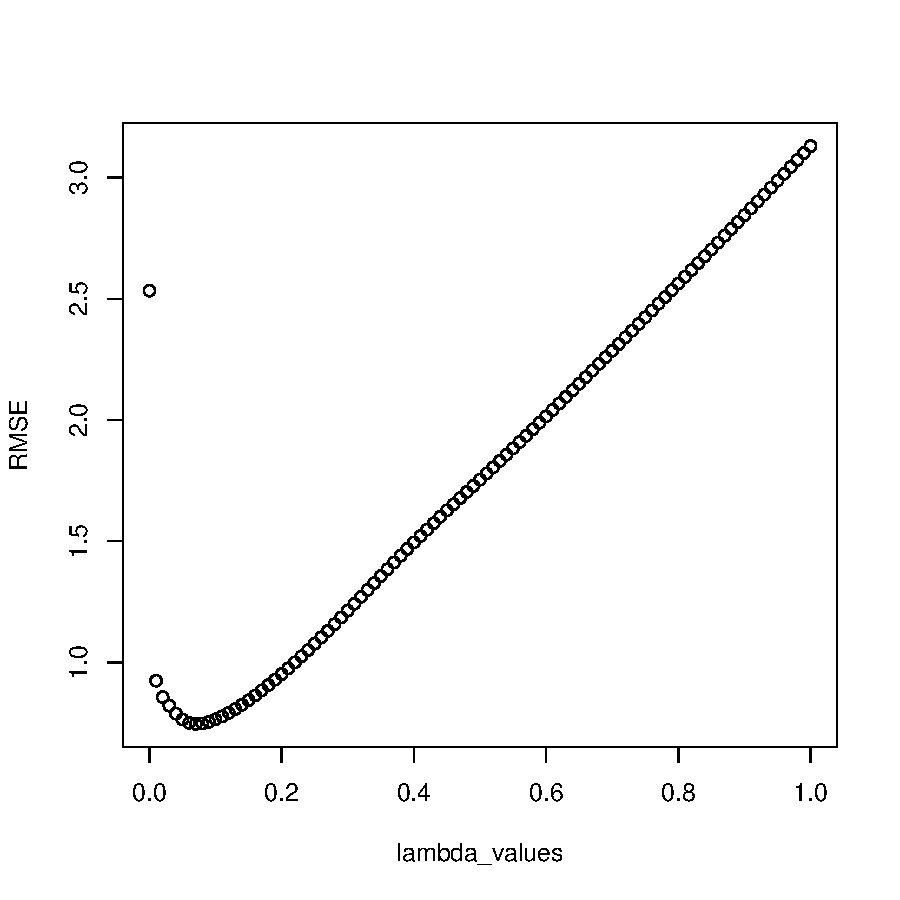
\includegraphics[width=\maxwidth]{figure/unnamed-chunk-21-1} \caption[RMSE for different lambda values]{RMSE for different lambda values}\label{fig:unnamed-chunk-21}
\end{figure}

\end{knitrout}

Based on the plot, the optimal lambda values seem to be between 0-0.2 somewhere. Hence, I will focus around there.

\begin{knitrout}
\definecolor{shadecolor}{rgb}{0.969, 0.969, 0.969}\color{fgcolor}\begin{kframe}
\begin{alltt}
\hlcom{#creating a sequence from 0 to 0.2 in 100 000 pieces. }
\hlstd{new_lambdas} \hlkwb{<-} \hlkwd{seq}\hlstd{(}\hlnum{0}\hlstd{,}\hlnum{0.2}\hlstd{,} \hlkwc{length.out} \hlstd{=} \hlnum{100000}\hlstd{)}
\hlstd{new_lambda_cv} \hlkwb{<-} \hlkwd{cross_validation_parallel}\hlstd{(}\hlkwc{X}\hlstd{=X,} \hlkwc{y}\hlstd{=y,} \hlkwc{n_folds}\hlstd{=}\hlnum{10}\hlstd{,} \hlkwc{lambdas}\hlstd{=new_lambdas,}
                          \hlkwc{export_vec} \hlstd{=} \hlkwd{c}\hlstd{(}\hlstr{"X"}\hlstd{,} \hlstr{"y"}\hlstd{,} \hlstr{"cross_validation"}\hlstd{,}
                                         \hlstr{"glmnet"}\hlstd{,} \hlstr{"errors_func"}\hlstd{) )}

\hlcom{#find the minimum}
\hlkwd{which}\hlstd{(new_lambda_cv} \hlopt{==} \hlkwd{min}\hlstd{(new_lambda_cv[,}\hlnum{2}\hlstd{]),} \hlkwc{arr.ind} \hlstd{=} \hlnum{TRUE}\hlstd{)}
\hlstd{multi_res[}\hlnum{15}\hlstd{,]}
\end{alltt}
\end{kframe}
\end{knitrout}

Well, I will not run this function again... but from the result I found the lambda with the least RMSE by using:
\begin{knitrout}
\definecolor{shadecolor}{rgb}{0.969, 0.969, 0.969}\color{fgcolor}\begin{kframe}
\begin{alltt}
\hlkwd{which}\hlstd{(new_lambda_cv} \hlopt{==} \hlkwd{min}\hlstd{(new_lambda_cv[,}\hlnum{2}\hlstd{]),} \hlkwc{arr.ind} \hlstd{=} \hlnum{TRUE}\hlstd{)}
\end{alltt}
\end{kframe}
\end{knitrout}

\begin{knitrout}
\definecolor{shadecolor}{rgb}{0.969, 0.969, 0.969}\color{fgcolor}\begin{kframe}
\begin{alltt}
                               row col
lambda =  0.0717627176271763 35882   2
\end{alltt}
\end{kframe}
\end{knitrout}

and then the corresponding MSE by:
\begin{knitrout}
\definecolor{shadecolor}{rgb}{0.969, 0.969, 0.969}\color{fgcolor}\begin{kframe}
\begin{alltt}
new_lambda_cv[35882,]

 MSE      RMSE 
0.5612816 0.7456794 
\end{alltt}
\end{kframe}
\end{knitrout}

Hence based on the results, the best lambda value I can get is $\lambda=0.0717627176271763 $with an RMSE of $0.7456$ and MSE of $0.5613$. I would probably have gotten away with simply using $\lambda = 0.07$ but now since I have this with more decimals I might as well use it.  However, I do not know if it is correct or not, but each of the iterations of lambda uses the same seed, which in a way makes the differences purely due to the lambda value.

\subsection{2.7 Predictions on test set}
Now we fit the model according to the best lambda value and make predictions on the test data
\begin{knitrout}
\definecolor{shadecolor}{rgb}{0.969, 0.969, 0.969}\color{fgcolor}\begin{kframe}
\begin{alltt}
\hlstd{best_lambda_model} \hlkwb{<-} \hlkwd{glmnet}\hlstd{(}\hlkwc{x} \hlstd{= X,} \hlkwc{y}\hlstd{= y,} \hlkwc{family} \hlstd{=} \hlstr{"gaussian"}\hlstd{,}
                            \hlkwc{alpha}\hlstd{=}\hlnum{1}\hlstd{,} \hlkwc{lambda}\hlstd{=} \hlnum{0.0717627176271763}\hlstd{)}
\hlstd{predictions} \hlkwb{<-} \hlkwd{predict}\hlstd{(best_lambda_model,} \hlkwc{newx} \hlstd{= X_test,} \hlkwc{type}\hlstd{=}\hlstr{"response"}\hlstd{)}

\hlkwd{errors_func}\hlstd{(}\hlkwc{y}\hlstd{=y_test,} \hlkwc{pred}\hlstd{= predictions)}
\end{alltt}
\begin{verbatim}
$MSE
[1] 0.650763

$RMSE
[1] 0.8066988
\end{verbatim}
\begin{alltt}
\hlcom{#just to compare that it gives the same results}
\hlstd{uuml}\hlopt{::}\hlkwd{rmse}\hlstd{(y_test, predictions)}
\end{alltt}
\begin{verbatim}
[1] 0.8066988
\end{verbatim}
\end{kframe}
\end{knitrout}
The RMSE is about 0.807 for the test set. 


\section{Task 3: Implementation of the Adam optimizer}
\subsection{3.1}
For this task we want to implement the Adam algorithm. Since we already have code for the different gradient descents algorithms ,we can just reuse parts of that code as well as the same plot functions which have been modified to keep the values of the betas into account. 


\begin{knitrout}
\definecolor{shadecolor}{rgb}{0.969, 0.969, 0.969}\color{fgcolor}\begin{kframe}
\begin{alltt}
\hlstd{Adam} \hlkwb{<-} \hlkwa{function}\hlstd{(}\hlkwc{y}\hlstd{,} \hlkwc{X}\hlstd{,} \hlkwc{eta} \hlstd{=} \hlnum{0.001}\hlstd{,} \hlkwc{B1} \hlstd{=} \hlnum{0.9}\hlstd{,} \hlkwc{B2} \hlstd{=} \hlnum{0.999}\hlstd{,}
                 \hlkwc{epsilon} \hlstd{=} \hlnum{10}\hlopt{^-}\hlnum{8}\hlstd{,} \hlkwc{theta} \hlstd{=} \hlkwd{rep}\hlstd{(}\hlnum{0}\hlstd{,} \hlkwd{ncol}\hlstd{(X)),} \hlkwc{epochs}\hlstd{,} \hlkwc{seed}\hlstd{=}\hlnum{1337}\hlstd{)\{}
  \hlstd{assertthat}\hlopt{::}\hlkwd{assert_that}\hlstd{(}\hlkwd{length}\hlstd{(y)} \hlopt{==} \hlkwd{nrow}\hlstd{(X),} \hlkwc{msg}\hlstd{=}\hlstr{"y and X length differ"}\hlstd{)}
  \hlstd{assertthat}\hlopt{::}\hlkwd{assert_that}\hlstd{(( B1} \hlopt{>=} \hlnum{0} \hlopt{&} \hlstd{B1} \hlopt{<} \hlnum{1}\hlstd{)} \hlopt{&} \hlstd{(B2} \hlopt{>=}\hlnum{0} \hlopt{&} \hlstd{B1} \hlopt{<}\hlnum{1} \hlstd{),}
                          \hlkwc{msg} \hlstd{=} \hlstr{"invalid Beta value"}\hlstd{)}
  \hlkwd{set.seed}\hlstd{(seed)}

  \hlstd{results} \hlkwb{<-} \hlkwd{matrix}\hlstd{(}\hlnum{0.0}\hlstd{,} \hlkwc{ncol} \hlstd{=} \hlkwd{ncol}\hlstd{(X)} \hlopt{+} \hlnum{2L}\hlstd{,} \hlkwc{nrow} \hlstd{= epochs)}
  \hlkwd{colnames}\hlstd{(results)} \hlkwb{<-} \hlkwd{c}\hlstd{(}\hlstr{"epoch"}\hlstd{,} \hlstr{"nll"}\hlstd{,} \hlkwd{colnames}\hlstd{(X))}

  \hlstd{m} \hlkwb{<-} \hlnum{0} \hlcom{#initalise 1st moment vector}
  \hlstd{v} \hlkwb{<-} \hlnum{0} \hlcom{#initalize 2nd moment vector}

  \hlkwa{for} \hlstd{(epoch} \hlkwa{in} \hlnum{1}\hlopt{:}\hlstd{epochs) \{}
      \hlstd{index_order} \hlkwb{<-} \hlkwd{sample}\hlstd{(}\hlkwd{length}\hlstd{(y))}
      \hlstd{X} \hlkwb{<-} \hlstd{X[index_order,]}
      \hlstd{y} \hlkwb{<-} \hlstd{y[index_order]}

      \hlcom{#shuffle the data by indexing in a random order}
    \hlstd{gradient} \hlkwb{<-} \hlopt{-}\hlkwd{ll_grad}\hlstd{(y, X, theta)} \hlcom{# neg.gradients w.r.t. stochastic objective at timestep t}

    \hlstd{m} \hlkwb{<-} \hlstd{B1}\hlopt{*}\hlstd{m} \hlopt{+} \hlstd{(}\hlnum{1}\hlopt{-}\hlstd{B1)}\hlopt{*}\hlstd{gradient} \hlcom{# Update biased first moment estimate)}
    \hlstd{v} \hlkwb{<-} \hlstd{B2}\hlopt{*}\hlstd{v} \hlopt{+} \hlstd{(}\hlnum{1}\hlopt{-}\hlstd{B2)}\hlopt{*}\hlstd{gradient}\hlopt{^}\hlnum{2} \hlcom{# Update biased second raw moment estimate)}

    \hlstd{m_hat} \hlkwb{<-} \hlstd{m}\hlopt{/}\hlstd{(}\hlnum{1}\hlopt{-}\hlstd{B1}\hlopt{^}\hlstd{epoch)} \hlcom{# Compute bias-corrected first moment estimate)}

    \hlstd{v_hat} \hlkwb{<-} \hlstd{v}\hlopt{/}\hlstd{(}\hlnum{1}\hlopt{-}\hlstd{B2}\hlopt{^}\hlstd{epoch)} \hlcom{#Compute bias-corrected second raw moment estimate)}

    \hlstd{theta} \hlkwb{<-} \hlstd{theta} \hlopt{-} \hlstd{( eta} \hlopt{*}\hlstd{m_hat} \hlopt{/} \hlstd{(} \hlkwd{sqrt}\hlstd{(v_hat)} \hlopt{+} \hlstd{epsilon) )}
    \hlcom{# Update parameters)}

    \hlstd{results[epoch,} \hlstr{"epoch"}\hlstd{]} \hlkwb{<-} \hlstd{epoch}
    \hlstd{results[epoch,} \hlstr{"nll"}\hlstd{]} \hlkwb{<-} \hlkwd{ll}\hlstd{(y, X, theta)}
    \hlstd{results[epoch,} \hlopt{-}\hlstd{(}\hlnum{1}\hlopt{:}\hlnum{2}\hlstd{)]} \hlkwb{<-} \hlstd{theta}
  \hlstd{\}}
  \hlkwd{attributes}\hlstd{(results)}\hlopt{$}\hlstd{B1} \hlkwb{<-} \hlstd{B1}
  \hlkwd{attributes}\hlstd{(results)}\hlopt{$}\hlstd{B2} \hlkwb{<-} \hlstd{B2}
  \hlkwd{attributes}\hlstd{(results)}\hlopt{$}\hlstd{learn_rate}\hlkwb{<-}\hlstd{eta}
  \hlkwd{attributes}\hlstd{(results)}\hlopt{$}\hlstd{epochs} \hlkwb{<-} \hlstd{epochs}
  \hlkwd{return}\hlstd{(results)}
\hlstd{\}}
\end{alltt}
\end{kframe}
\end{knitrout}
\subsection{3.2}
\begin{knitrout}
\definecolor{shadecolor}{rgb}{0.969, 0.969, 0.969}\color{fgcolor}\begin{kframe}
\begin{alltt}
\hlkwd{print}\hlstd{(Adam)}
\end{alltt}
\begin{verbatim}
function(y, X, eta = 0.001, B1 = 0.9, B2 = 0.999,
                 epsilon = 10^-8, theta = rep(0, ncol(X)), epochs, seed=1337){
  assertthat::assert_that(length(y) == nrow(X), msg="y and X length differ")
  assertthat::assert_that(( B1 >= 0 & B1 < 1) & (B2 >=0 & B1 <1 ), 
                          msg = "invalid Beta value")
  set.seed(seed)
  
  results <- matrix(0.0, ncol = ncol(X) + 2L, nrow = epochs)
  colnames(results) <- c("epoch", "nll", colnames(X))
  
  m <- 0 #initalise 1st moment vector
  v <- 0 #initalize 2nd moment vector
  
  for (epoch in 1:epochs) { 
      index_order <- sample(length(y))
      X <- X[index_order,]
      y <- y[index_order]
      
      #shuffle the data by indexing in a random order
    gradient <- -ll_grad(y, X, theta) # neg.gradients w.r.t. stochastic objective at timestep t
     
    m <- B1*m + (1-B1)*gradient # Update biased first moment estimate)
    v <- B2*v + (1-B2)*gradient^2 # Update biased second raw moment estimate)
    
    m_hat <- m/(1-B1^epoch) # Compute bias-corrected first moment estimate)
    
    v_hat <- v/(1-B2^epoch) #Compute bias-corrected second raw moment estimate)
    
    theta <- theta - ( eta *m_hat / ( sqrt(v_hat) + epsilon) ) 
    # Update parameters)
    
    results[epoch, "epoch"] <- epoch
    results[epoch, "nll"] <- ll(y, X, theta)
    results[epoch, -(1:2)] <- theta
  }
  attributes(results)$B1 <- B1
  attributes(results)$B2 <- B2
  attributes(results)$learn_rate<-eta
  attributes(results)$epochs <- epochs
  return(results)
}
\end{verbatim}
\end{kframe}
\end{knitrout}

\subsection{3.3}
First we generalize the function:
\begin{knitrout}
\definecolor{shadecolor}{rgb}{0.969, 0.969, 0.969}\color{fgcolor}\begin{kframe}
\begin{alltt}
\hlstd{Adam_multi} \hlkwb{<-} \hlkwa{function}\hlstd{(}\hlkwc{y}\hlstd{,} \hlkwc{X}\hlstd{,} \hlkwc{etas}\hlstd{,} \hlkwc{B1s}\hlstd{,} \hlkwc{B2s}\hlstd{,} \hlkwc{epsilon}\hlstd{,} \hlkwc{theta}\hlstd{,} \hlkwc{epochs}\hlstd{,} \hlkwc{seed}\hlstd{)\{}
  \hlstd{result_list} \hlkwb{<-} \hlkwd{mapply}\hlstd{(}\hlkwc{FUN} \hlstd{= Adam, etas, B1s, B2s,}
         \hlkwc{MoreArgs} \hlstd{=} \hlkwd{list}\hlstd{(}\hlkwc{y} \hlstd{= y,} \hlkwc{X} \hlstd{= X,} \hlkwc{epsilon} \hlstd{= epsilon,}
                         \hlkwc{theta} \hlstd{= theta,} \hlkwc{epochs} \hlstd{= epochs,} \hlkwc{seed} \hlstd{= seed),}
         \hlkwc{SIMPLIFY} \hlstd{=} \hlnum{FALSE}\hlstd{)}
  \hlkwd{return}\hlstd{(result_list)}
\hlstd{\}}


\hlstd{task_3_main} \hlkwb{<-} \hlkwa{function}\hlstd{(}\hlkwc{y}\hlstd{,} \hlkwc{X}\hlstd{,} \hlkwc{etas}\hlstd{,} \hlkwc{B1s}\hlstd{,} \hlkwc{B2s}\hlstd{,}
                        \hlkwc{theta} \hlstd{=} \hlkwd{rep}\hlstd{(}\hlnum{0}\hlstd{,} \hlkwd{ncol}\hlstd{(X)),} \hlkwc{epochs} \hlstd{=} \hlnum{500}\hlstd{,}
                        \hlkwc{epsilon}\hlstd{=} \hlnum{10}\hlopt{^-}\hlnum{8}\hlstd{,} \hlkwc{seed}\hlstd{=}\hlnum{1337}\hlstd{,} \hlkwc{variable_name}\hlstd{)\{}

 \hlstd{res} \hlkwb{<-}  \hlkwd{Adam_multi}\hlstd{(}\hlkwc{y}\hlstd{=y,} \hlkwc{X}\hlstd{=X,} \hlkwc{etas} \hlstd{= etas,} \hlkwc{B1s} \hlstd{= B1s,} \hlkwc{B2s} \hlstd{= B2s,}\hlkwc{theta} \hlstd{= theta,}
             \hlkwc{epsilon} \hlstd{= epsilon,} \hlkwc{epochs}\hlstd{=epochs,} \hlkwc{seed}\hlstd{=seed)}
 \hlstd{plots} \hlkwb{<-} \hlkwd{plot_GD_multi}\hlstd{(res, variable_name)}
 \hlkwd{return}\hlstd{(}\hlkwd{list}\hlstd{(res, plots))}
\hlstd{\}}
\end{alltt}
\end{kframe}
\end{knitrout}

Now we just try some different combinations of the values for $\eta, \beta_1, \beta_2$. 
\begin{knitrout}
\definecolor{shadecolor}{rgb}{0.969, 0.969, 0.969}\color{fgcolor}\begin{kframe}
\begin{alltt}
\hlstd{etas_vec} \hlkwb{=} \hlkwd{c}\hlstd{(}\hlnum{0.001}\hlstd{,} \hlnum{0.1}\hlstd{,} \hlnum{1}\hlstd{)}
\hlstd{Beta_ones} \hlkwb{<-} \hlkwd{c}\hlstd{(}\hlnum{0.9}\hlstd{,} \hlnum{0.85}\hlstd{,} \hlnum{0.5}\hlstd{)}
\hlstd{Beta_twos} \hlkwb{<-} \hlkwd{c}\hlstd{(}\hlnum{0.999}\hlstd{,} \hlnum{0.95}\hlstd{,} \hlnum{0.8}\hlstd{)}
\hlstd{X} \hlkwb{<-} \hlkwd{model.matrix}\hlstd{(admit} \hlopt{~} \hlstd{gre_sd} \hlopt{+} \hlstd{gpa_sd, binary)}
\hlstd{y} \hlkwb{<-} \hlstd{binary}\hlopt{$}\hlstd{admit}

\hlstd{adam_results} \hlkwb{<-} \hlkwd{task_3_main}\hlstd{(}\hlkwc{y}\hlstd{=y,} \hlkwc{X}\hlstd{=X,} \hlkwc{etas} \hlstd{= etas_vec,}
            \hlkwc{B1s} \hlstd{= Beta_ones,} \hlkwc{B2s} \hlstd{= Beta_twos,} \hlkwc{variable_name} \hlstd{=} \hlstr{"gre_sd"} \hlstd{)}
\end{alltt}
\end{kframe}
\end{knitrout}

\begin{knitrout}
\definecolor{shadecolor}{rgb}{0.969, 0.969, 0.969}\color{fgcolor}\begin{kframe}
\begin{alltt}
\hlkwd{plot}\hlstd{(adam_results[[}\hlnum{2}\hlstd{]])}
\end{alltt}
\end{kframe}\begin{figure}
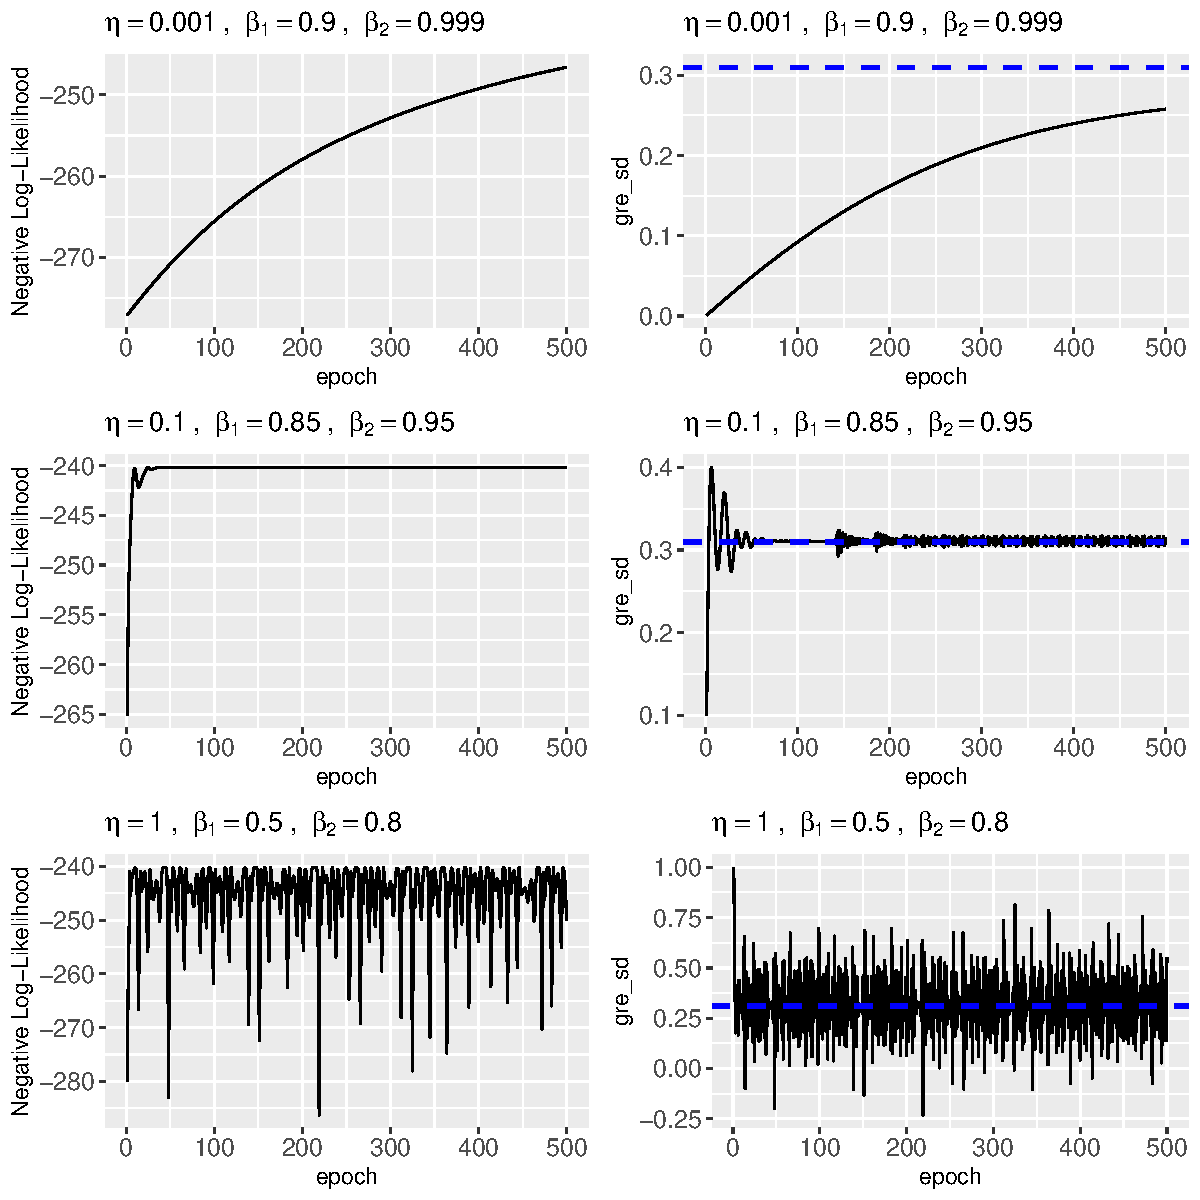
\includegraphics[width=\maxwidth]{figure/adam_results-1} \caption[Results for Adam implementation]{Results for Adam implementation}\label{fig:adam_results}
\end{figure}

\end{knitrout}

The results are seen in figure \ref{fig:adam_results}. The first combination is simply the recommended default settings as proposed by Kingma \& Ba (2015). And as can be seen from the results, it does to to converge rather slowly as an exponential decay for this case. If we were to increase the number of epochs it looks like it would converge after around 1000-2000 epochs. 

In a similar way as in task 2.3, I chose the other combination of values of $\eta, \beta_1, \beta_2$ so that it would converge faster in one case, and diverge in the other. In order to adjust for that, it would seem rather natural to change the step size or learning rate $\eta$ as it is rather small. As for the hyper parameters $\beta_1$ and $\beta_2$, they control the exponential decay  of the moving averages of the gradient $m_t$ and squared gradient $v_t$. But i would not say that is obvious which values to choose such that it would converge faster or slower. So they were chosen by some trial and error. The second combination as can be seen in the plot, does converge rather well to the "true" value, albeit it is showing signs of slightly jumping around the "true" value, which is probably due to the changes in the hyper parameter and the effect of the moving averages. The last combination shows a scenario where it never converges. 

\section{Appendix: Additional R-code}
\subsection{Task 2.3}
\begin{knitrout}
\definecolor{shadecolor}{rgb}{0.969, 0.969, 0.969}\color{fgcolor}\begin{kframe}
\begin{alltt}
\hlcom{#' Function to plot negative log likelihood and the results for one chosen }
\hlcom{#' parameter}
\hlcom{#' @param results The results from either ordinary, stochastic, or minibatch }
\hlcom{#' gtadient descent. Also, later added support for Adam results. }
\hlcom{#' @param  variable_name name of the parameter to plot results for}
\hlcom{#' @return  plots for the negative log-likelihood as well as the parameter }
\hlcom{#' of interest}
\hlcom{#'}
\hlstd{plot_GD} \hlkwb{<-} \hlkwa{function}\hlstd{(}\hlkwc{results}\hlstd{,} \hlkwc{variable_name} \hlstd{)\{}
  \hlstd{variable_name} \hlcom{#this is just to instantiate the object within the local}
 \hlcom{# environment due to some weird bug later with the plot_GD_multi function }
  \hlstd{n_epochs} \hlkwb{<-} \hlkwd{attributes}\hlstd{(results)}\hlopt{$}\hlstd{epochs}
  \hlstd{learn_rate} \hlkwb{<-} \hlkwd{attributes}\hlstd{(results)}\hlopt{$}\hlstd{learn_rate}
  \hlstd{result_df} \hlkwb{<-} \hlkwd{data.frame}\hlstd{(results)}

\hlcom{# Check for Adam implementation attributes (added later).}
\hlstd{attributes_to_check} \hlkwb{<-} \hlkwd{c}\hlstd{(}\hlstr{"B1"}\hlstd{,} \hlstr{"B2"}\hlstd{)}

\hlkwa{if} \hlstd{(}\hlstr{"B1"} \hlopt \hlkwd{names}\hlstd{(}\hlkwd{attributes}\hlstd{(results))} \hlopt{&&} \hlstr{"B2"} \hlopt \hlkwd{names}\hlstd{(}\hlkwd{attributes}\hlstd{(results))) \{}
    \hlstd{B1} \hlkwb{<-} \hlkwd{attributes}\hlstd{(results)}\hlopt{$}\hlstd{B1}
    \hlstd{B2} \hlkwb{<-} \hlkwd{attributes}\hlstd{(results)}\hlopt{$}\hlstd{B2}
    \hlstd{title_text} \hlkwb{<-} \hlkwd{bquote}\hlstd{(eta} \hlopt{==} \hlkwd{.}\hlstd{(learn_rate)} \hlopt{~}
                           \hlstr{", "} \hlopt{~} \hlstd{beta[}\hlnum{1}\hlstd{]} \hlopt{==} \hlkwd{.}\hlstd{(B1)} \hlopt{~} \hlstr{", "} \hlopt{~} \hlstd{beta[}\hlnum{2}\hlstd{]} \hlopt{==} \hlkwd{.}\hlstd{(B2))}

  \hlstd{\}} \hlkwa{else} \hlstd{\{}
    \hlstd{title_text} \hlkwb{<-} \hlkwd{bquote}\hlstd{(eta} \hlopt{==} \hlkwd{.}\hlstd{(learn_rate))}
  \hlstd{\}}

\hlstd{y_var} \hlkwb{<-} \hlkwd{ensym}\hlstd{(variable_name)} \hlcom{# ensym + injection with !! to inject the variable}
\hlcom{#rather than the string provided by variable_name}

   \hlcom{#plot negative Log-likelihood}
   \hlstd{ll_plot} \hlkwb{<-} \hlkwd{ggplot}\hlstd{(result_df,} \hlkwd{aes}\hlstd{(}\hlkwc{x}\hlstd{=epoch,} \hlkwc{y}\hlstd{=nll))} \hlopt{+} \hlkwd{geom_line}\hlstd{()} \hlopt{+}
     \hlkwd{ylab}\hlstd{(}\hlstr{"Negative Log-Likelihood"}\hlstd{)} \hlopt{+}
     \hlkwd{ggtitle}\hlstd{(title_text)} \hlopt{+}
     \hlkwd{theme}\hlstd{(}\hlkwc{axis.text} \hlstd{=} \hlkwd{element_text}\hlstd{(}\hlkwc{size} \hlstd{=} \hlnum{12}\hlstd{))}
  \hlstd{variable_plot} \hlkwb{<-}   \hlkwd{ggplot}\hlstd{(result_df,} \hlkwd{aes}\hlstd{(}\hlkwc{x} \hlstd{= epoch,}
                                           \hlkwc{y} \hlstd{=} \hlopt{!!}\hlstd{y_var))} \hlopt{+}
    \hlkwd{geom_line}\hlstd{()} \hlopt{+}
    \hlkwd{geom_hline}\hlstd{(}\hlkwc{yintercept} \hlstd{=} \hlnum{0.31}\hlstd{,} \hlkwc{col}\hlstd{=}\hlstr{"blue"}\hlstd{,}\hlkwc{linewidth}\hlstd{=}\hlnum{1}\hlstd{,} \hlkwc{linetype} \hlstd{=} \hlstr{"dashed"}\hlstd{)} \hlopt{+}
    \hlkwd{ggtitle}\hlstd{(title_text)} \hlopt{+}
    \hlkwd{theme}\hlstd{(}\hlkwc{axis.text} \hlstd{=} \hlkwd{element_text}\hlstd{(}\hlkwc{size} \hlstd{=} \hlnum{12}\hlstd{))}

   \hlstd{plots} \hlkwb{<-} \hlkwd{grid.arrange}\hlstd{(ll_plot, variable_plot,} \hlkwc{ncol}\hlstd{=}\hlnum{2}\hlstd{)}
  \hlkwd{return}\hlstd{(plots)}
\hlstd{\}}
\end{alltt}
\end{kframe}
\end{knitrout}

\begin{knitrout}
\definecolor{shadecolor}{rgb}{0.969, 0.969, 0.969}\color{fgcolor}\begin{kframe}
\begin{alltt}
\hlcom{#' wrapper functions to make the previous functions more}
\hlcom{#'  generalized to multiple values of learn_rates}
\hlcom{#' @param learn_rates a vector of different learning rates to try. }
\hlcom{#' All other arguments are the same}

\hlstd{batch_gsd_multi} \hlkwb{<-} \hlkwa{function}\hlstd{(}\hlkwc{y}\hlstd{,} \hlkwc{X}\hlstd{,} \hlkwc{learn_rates}\hlstd{,}
                            \hlkwc{thetas} \hlstd{=} \hlkwd{rep}\hlstd{(}\hlnum{0}\hlstd{,} \hlkwd{ncol}\hlstd{(X)),} \hlkwc{n_epochs}\hlstd{)\{}
  \hlstd{res} \hlkwb{<-} \hlkwd{mapply}\hlstd{(}\hlkwc{FUN} \hlstd{= batch_gsd,} \hlkwc{learn_rate}\hlstd{=learn_rates,}
                \hlkwc{MoreArgs} \hlstd{=} \hlkwd{list}\hlstd{(}\hlkwc{y}\hlstd{=y,} \hlkwc{X}\hlstd{=X,}
                                \hlkwc{theta} \hlstd{= thetas,} \hlkwc{epochs} \hlstd{= n_epochs),}
                \hlkwc{SIMPLIFY} \hlstd{=} \hlnum{FALSE}\hlstd{)}
\hlkwd{return}\hlstd{(res)}
\hlstd{\}}

\hlstd{stochastic_gsd_multi} \hlkwb{<-} \hlkwa{function}\hlstd{(}\hlkwc{y}\hlstd{,} \hlkwc{X}\hlstd{,} \hlkwc{learn_rates}\hlstd{,}
                                 \hlkwc{thetas} \hlstd{=} \hlkwd{rep}\hlstd{(}\hlnum{0}\hlstd{,} \hlkwd{ncol}\hlstd{(X)),} \hlkwc{n_epochs}\hlstd{,} \hlkwc{seed}\hlstd{=}\hlnum{1337}\hlstd{)\{}
  \hlstd{res} \hlkwb{<-} \hlkwd{mapply}\hlstd{(}\hlkwc{FUN} \hlstd{= stochastic_gsd,} \hlkwc{learn_rate}\hlstd{=learn_rates,}
                \hlkwc{MoreArgs} \hlstd{=} \hlkwd{list}\hlstd{(}\hlkwc{y}\hlstd{=y,} \hlkwc{X}\hlstd{=X,}
                                \hlkwc{theta} \hlstd{= thetas,} \hlkwc{epochs} \hlstd{= n_epochs,}
                                \hlkwc{seed}\hlstd{=seed),}
                \hlkwc{SIMPLIFY} \hlstd{=} \hlnum{FALSE}\hlstd{)}
  \hlkwd{return}\hlstd{(res)}
\hlstd{\}}

\hlstd{minibatch_gsd_multi} \hlkwb{<-} \hlkwa{function}\hlstd{(}\hlkwc{y}\hlstd{,} \hlkwc{X}\hlstd{,} \hlkwc{learn_rates}\hlstd{,}
                                 \hlkwc{thetas} \hlstd{=} \hlkwd{rep}\hlstd{(}\hlnum{0}\hlstd{,} \hlkwd{ncol}\hlstd{(X)),} \hlkwc{n_epochs}\hlstd{,}
                                \hlkwc{seed}\hlstd{=}\hlnum{1337}\hlstd{,} \hlkwc{batch_size}\hlstd{) \{}

  \hlstd{res} \hlkwb{<-} \hlkwd{mapply}\hlstd{(}\hlkwc{FUN} \hlstd{= minibatch_gsd,} \hlkwc{learn_rate}\hlstd{=learn_rates,}
                \hlkwc{MoreArgs} \hlstd{=} \hlkwd{list}\hlstd{(}\hlkwc{y}\hlstd{=y,} \hlkwc{X}\hlstd{=X,}
                                \hlkwc{theta} \hlstd{= thetas,} \hlkwc{epochs} \hlstd{= n_epochs,}
                                \hlkwc{seed}\hlstd{=seed,} \hlkwc{batch_size} \hlstd{= batch_size),}
                \hlkwc{SIMPLIFY} \hlstd{=} \hlnum{FALSE}\hlstd{)}
  \hlkwd{return}\hlstd{(res)}
  \hlstd{\}}


\hlcom{#' function to generalize the plot_GD function to multiple plots in the same grid}

\hlstd{plot_GD_multi} \hlkwb{<-}\hlkwa{function}\hlstd{(}\hlkwc{results_list}\hlstd{,} \hlkwc{variable_name}\hlstd{)\{}
  \hlstd{extracted_plots} \hlkwb{<-} \hlkwd{lapply}\hlstd{(results_list,} \hlkwc{FUN}\hlstd{= plot_GD,}
                            \hlkwc{variable_name} \hlstd{= variable_name)}

  \hlstd{merged_plots} \hlkwb{<-} \hlkwd{do.call}\hlstd{(grid.arrange,} \hlkwd{c}\hlstd{(extracted_plots,}
                                          \hlkwc{nrow}\hlstd{=}\hlkwd{length}\hlstd{(extracted_plots)))}
  \hlcom{#using grid.arrange on all extracted plots}
  \hlkwd{return}\hlstd{(merged_plots)}
\hlstd{\}}
\end{alltt}
\end{kframe}
\end{knitrout}

\begin{knitrout}
\definecolor{shadecolor}{rgb}{0.969, 0.969, 0.969}\color{fgcolor}\begin{kframe}
\begin{alltt}
\hlstd{Task_3_main} \hlkwb{<-} \hlkwa{function}\hlstd{(}\hlkwc{y}\hlstd{,} \hlkwc{X}\hlstd{,} \hlkwc{thetas} \hlstd{=} \hlkwd{rep}\hlstd{(}\hlnum{0}\hlstd{,} \hlkwd{ncol}\hlstd{(X)) ,} \hlkwc{learn_rates}\hlstd{,}
                        \hlkwc{n_epochs}\hlstd{,} \hlkwc{seed}\hlstd{,} \hlkwc{batch_size}\hlstd{,} \hlkwc{variable_name}\hlstd{)\{}

\hlstd{batch_results} \hlkwb{<-} \hlkwd{batch_gsd_multi}\hlstd{(}\hlkwc{y} \hlstd{= y,} \hlkwc{X}\hlstd{=X,}
                                 \hlkwc{learn_rates} \hlstd{= learn_rates[[}\hlnum{1}\hlstd{]],}
                                 \hlkwc{n_epochs} \hlstd{=} \hlnum{500}\hlstd{,} \hlkwc{thetas}\hlstd{=thetas)}
\hlkwd{print}\hlstd{(}\hlstr{"Ordinary GD done"}\hlstd{)}

\hlstd{stochastic_results} \hlkwb{<-} \hlkwd{stochastic_gsd_multi}\hlstd{(}\hlkwc{y} \hlstd{= y,} \hlkwc{X}\hlstd{=X,}
                                           \hlkwc{learn_rates} \hlstd{= learn_rates[[}\hlnum{2}\hlstd{]],}
                                           \hlkwc{n_epochs} \hlstd{= n_epochs,} \hlkwc{seed}\hlstd{=seed)}
\hlkwd{print}\hlstd{(}\hlstr{"Stochastic GD done"}\hlstd{)}

\hlstd{minibatch_results} \hlkwb{<-}  \hlkwd{minibatch_gsd_multi}\hlstd{(}\hlkwc{y} \hlstd{= y,} \hlkwc{X}\hlstd{=X,}
                                          \hlkwc{learn_rates} \hlstd{= learn_rates[[}\hlnum{3}\hlstd{]],}
                                          \hlkwc{n_epochs} \hlstd{= n_epochs,}
                                          \hlkwc{batch_size}\hlstd{=batch_size,}
                                          \hlkwc{seed}\hlstd{=seed)}
\hlkwd{print}\hlstd{(}\hlstr{"Minibatch GD done"}\hlstd{)}
\hlstd{batch_plots} \hlkwb{<-} \hlkwd{plot_GD_multi}\hlstd{(batch_results,}
                             \hlkwc{variable_name} \hlstd{= variable_name)}
\hlstd{stochastic_plots} \hlkwb{<-} \hlkwd{plot_GD_multi}\hlstd{(stochastic_results,}
                                  \hlkwc{variable_name} \hlstd{= variable_name)}
\hlstd{minibatch_plots} \hlkwb{<-} \hlkwd{plot_GD_multi}\hlstd{(minibatch_results,}
                                 \hlkwc{variable_name} \hlstd{= variable_name)}
\hlstd{list_results} \hlkwb{<-} \hlkwd{list}\hlstd{(}\hlkwc{batch_GD} \hlstd{=batch_plots,}
                     \hlkwc{stochastic_GD} \hlstd{= stochastic_plots,}
                     \hlkwc{minibatch_GD} \hlstd{= minibatch_plots)}
\hlkwd{return}\hlstd{(list_results)}
\hlstd{\}}
\end{alltt}
\end{kframe}
\end{knitrout}
\end{document}

\subsection{3.2 lasso }

The regularization methods shrinks the coefficients by a penalty term $\lambda$ .
The \texttt{cv.glmnet()} function is a cross-validation version of the function \texttt{glm.net()}, where the latter one works by fitting the penalized maximum likelihood glm-model with the specified elastic mixing parameter $\alpha$. If $\alpha=1$, which is the value we use in this case,  then its the the lasso penalty and if $\alpha = 0$ then it is the ridge penalty. 
The function performs  k-fold cross validation for glmnet and returns a value for $\lambda$ . The cv-glmnet works   by first  running the glmnet the get the lambda sequence. After that, for each fold that is not included it calculates the fit. Hence the returned object is a list with all the results from the cross-validation fit.
\begin{knitrout}
\definecolor{shadecolor}{rgb}{0.969, 0.969, 0.969}\color{fgcolor}\begin{kframe}
\begin{alltt}
\hlkwd{library}\hlstd{(uuml)}
\hlkwd{data}\hlstd{(}\hlstr{"prob2_train"}\hlstd{)}
\hlkwd{data}\hlstd{(}\hlstr{"prob2_test"}\hlstd{)}
\hlkwd{dim}\hlstd{(prob2_train)}

\hlstd{lasso_cv}\hlkwb{<-} \hlkwd{cv.glmnet}\hlstd{(}\hlkwc{y}\hlstd{= prob2_train}\hlopt{$}\hlstd{y,} \hlkwc{x}\hlstd{=} \hlkwd{as.matrix}\hlstd{(}\hlkwc{x}\hlstd{= prob2_train[,}\hlnum{1}\hlopt{:}\hlnum{240}\hlstd{]),}
          \hlkwc{family}\hlstd{=}\hlstr{"gaussian"}\hlstd{,}
                             \hlkwc{alpha}\hlstd{=}\hlnum{1}\hlstd{)}
\end{alltt}
\end{kframe}
\end{knitrout}

Now to plot the results.
\begin{knitrout}
\definecolor{shadecolor}{rgb}{0.969, 0.969, 0.969}\color{fgcolor}\begin{kframe}
\begin{alltt}
\hlkwd{plot}\hlstd{(lasso_cv)}
\hlkwd{print}\hlstd{(lasso_cv}\hlopt{$}\hlstd{lambda.min)}
\hlkwd{print}\hlstd{(lasso_cv}\hlopt{$}\hlstd{lambda.1se)}
\end{alltt}
\end{kframe}
\end{knitrout}
In figure \ref{fig:lasso_plot} the x-axis is the (log) $\lambda$-sequence and the y-axis the mean square error for the different values. It shows the cross-validation curve as the red dots as well as the curves for both the upper standard deviation and lower standard deviation. There are also two vertical lines, where one is the \texttt{lambda.min()}-value such that it is the value of $lambda$ which yields the smallest MSE, while the other vertical line is the \texttt{lambda.1se} value which corresponds to the value of $\lambda$ that yields the most regularized model in the sense that the cross-validation error is within 1 standard error of the minimum. 

\subsection{3.3 lasso coefficients}
Now we want to look at the coefficients from the $\lambda_{\text[min]}$ and $\lambda_{1 \text{se}}$-models.

\begin{knitrout}
\definecolor{shadecolor}{rgb}{0.969, 0.969, 0.969}\color{fgcolor}\begin{kframe}
\begin{alltt}
\hlstd{lasso_coeffs} \hlkwb{<-} \hlkwd{coef}\hlstd{(lasso_cv,} \hlkwc{s}\hlstd{=}\hlstr{"lambda.min"}\hlstd{)}
\end{alltt}
\end{kframe}
\end{knitrout}
The object \texttt{coeffs} contains all the coefficients of the variables in a sparse format which are from the model corresponding to the minimum lambda value. if we just look at the first and last values it looks like this:
\begin{knitrout}
\definecolor{shadecolor}{rgb}{0.969, 0.969, 0.969}\color{fgcolor}\begin{kframe}
\begin{alltt}
\hlkwd{head}\hlstd{(lasso_coeffs)}
\hlkwd{tail}\hlstd{(lasso_coeffs)}
\end{alltt}
\end{kframe}
\end{knitrout}
where the coefficients not used has a value of 0 represented by the dot. We can extract only the variables with non-zero values with this:
\begin{knitrout}
\definecolor{shadecolor}{rgb}{0.969, 0.969, 0.969}\color{fgcolor}\begin{kframe}
\begin{alltt}
\hlstd{used_coefs} \hlkwb{<-} \hlstd{lasso_coeffs[lasso_coeffs}\hlopt{@}\hlkwc{i}\hlopt{+}\hlnum{1}\hlstd{,]} \hlcom{#@ due to S4 class}
\hlkwd{print}\hlstd{(used_coefs)}
\hlkwd{length}\hlstd{(used_coefs)}
\end{alltt}
\end{kframe}
\end{knitrout}
Hence, only 16 variables were used for this model.

Now we do the same thing for the \texttt{se1} model. 
\begin{knitrout}
\definecolor{shadecolor}{rgb}{0.969, 0.969, 0.969}\color{fgcolor}\begin{kframe}
\begin{alltt}
\hlstd{lasso_coeffs_se} \hlkwb{<-} \hlkwd{coef}\hlstd{(lasso_cv,} \hlkwc{s}\hlstd{=}\hlstr{"lambda.1se"}\hlstd{)}
\hlstd{lasso_coeffs_se[lasso_coeffs_se}\hlopt{@}\hlkwc{i}\hlopt{+}\hlnum{1}\hlstd{,]} \hlopt
  \hlkwd{print}\hlstd{()}
\end{alltt}
\end{kframe}
\end{knitrout}
This model contains slightly less variables with 13 variables used. However, the variables used here are also used for the previous model due to both containing V1-V10, V17, V88 and V222 with  the very similar, but not exactly the same, values for the coefficients. 

\subsection{3.4 ridge regression}
Now we fit a ridge regression the same way as before but by setting the $\alpha$-argument to 0.
\begin{knitrout}
\definecolor{shadecolor}{rgb}{0.969, 0.969, 0.969}\color{fgcolor}\begin{kframe}
\begin{alltt}
\hlstd{ridge_cv} \hlkwb{<-} \hlkwd{cv.glmnet}\hlstd{(}\hlkwc{y}\hlstd{= prob2_train}\hlopt{$}\hlstd{y,} \hlkwc{x}\hlstd{=} \hlkwd{as.matrix}\hlstd{(}\hlkwc{x}\hlstd{= prob2_train[,}\hlnum{1}\hlopt{:}\hlnum{240}\hlstd{]),}
          \hlkwc{family}\hlstd{=}\hlstr{"gaussian"}\hlstd{,}
                             \hlkwc{alpha}\hlstd{=}\hlnum{0}\hlstd{)}
\hlkwd{plot}\hlstd{(ridge_cv)}

\hlstd{ridge_cv}\hlopt{$}\hlstd{lambda.min}
\hlstd{ridge_cv}\hlopt{$}\hlstd{lambda.1se}
\end{alltt}
\end{kframe}
\end{knitrout}

\subsection{3.5 predictions}
To make predictions we use the lambda values which we found for the models. To make the predictions we use the \texttt{predict()} function together with the models contained within the \texttt{lasso\_cv} and \texttt{ridge\_cv} objects, rather than fitting a new model with the corresponding lambda values. Since in the first case we provided the whole lambda sequence and get a moving start, which provides slightly different but better estimates.  
\begin{knitrout}
\definecolor{shadecolor}{rgb}{0.969, 0.969, 0.969}\color{fgcolor}\begin{kframe}
\begin{alltt}
\hlstd{lasso_min} \hlkwb{<-} \hlkwd{predict}\hlstd{(lasso_cv,} \hlkwc{type} \hlstd{=} \hlstr{"response"}\hlstd{,} \hlkwc{s} \hlstd{= lasso_cv}\hlopt{$}\hlstd{lambda.min,}
                     \hlkwc{newx}\hlstd{=}\hlkwd{as.matrix}\hlstd{(prob2_test[,}\hlnum{1}\hlopt{:}\hlnum{240}\hlstd{]))}
\hlcom{#' function to make predictions for a cv_fit object with lambda.min and lamda.1se}
\hlstd{predict_func} \hlkwb{<-} \hlkwa{function}\hlstd{(}\hlkwc{cv_fit}\hlstd{,} \hlkwc{type} \hlstd{=} \hlstr{"response"}\hlstd{,} \hlkwc{newx}\hlstd{)\{}
  \hlstd{newx} \hlkwb{<-} \hlkwd{as.matrix}\hlstd{(newx)}

  \hlstd{y_preds_min_lambda} \hlkwb{<-} \hlkwd{predict}\hlstd{(cv_fit,} \hlkwc{type}\hlstd{=type,}
                                \hlkwc{s}\hlstd{=cv_fit}\hlopt{$}\hlstd{lambda.min,} \hlkwc{newx}\hlstd{=newx )}

  \hlstd{y_preds_1se} \hlkwb{<-}  \hlkwd{predict}\hlstd{(cv_fit,} \hlkwc{type}\hlstd{=type,}
                          \hlkwc{s}\hlstd{=cv_fit}\hlopt{$}\hlstd{lambda.1se,} \hlkwc{newx}\hlstd{=newx)}

  \hlstd{results} \hlkwb{<-} \hlkwd{matrix}\hlstd{(}\hlkwc{data} \hlstd{=} \hlkwd{cbind}\hlstd{(y_preds_min_lambda, y_preds_1se),} \hlkwc{ncol}\hlstd{=}\hlnum{2}\hlstd{)}
  \hlkwd{colnames}\hlstd{(results)} \hlkwb{<-} \hlkwd{c}\hlstd{(}\hlstr{"lambda.min"}\hlstd{,} \hlstr{"lambda.1se"}\hlstd{)}
  \hlkwd{return}\hlstd{(results)}
\hlstd{\}}

\hlcom{#' function to calculate MSE and RMSE}
\hlstd{errors_func} \hlkwb{<-} \hlkwa{function}\hlstd{(}\hlkwc{y_obs}\hlstd{,} \hlkwc{pred}\hlstd{)\{}
  \hlstd{assertthat}\hlopt{::}\hlkwd{assert_that}\hlstd{(}\hlkwd{length}\hlstd{(y_obs)} \hlopt{==} \hlkwd{length}\hlstd{(pred),} \hlkwc{msg}\hlstd{=}\hlstr{"lengths differ"}\hlstd{)}
  \hlstd{n} \hlkwb{<-} \hlkwd{length}\hlstd{(y_obs)}
  \hlstd{Sum_square} \hlkwb{<-} \hlkwd{sum}\hlstd{( (y_obs} \hlopt{-} \hlstd{pred)}\hlopt{^}\hlnum{2}\hlstd{)}
  \hlstd{MSE} \hlkwb{<-} \hlstd{Sum_square} \hlopt{/} \hlstd{n}
  \hlstd{RMSE} \hlkwb{<-} \hlkwd{sqrt}\hlstd{(MSE)}
  \hlstd{res} \hlkwb{<-} \hlkwd{list}\hlstd{(}\hlstr{"MSE"}\hlstd{= MSE,} \hlstr{"RMSE"} \hlstd{= RMSE)}
  \hlkwd{return}\hlstd{(res)}
\hlstd{\}}

\hlcom{#' both functions combined given a cv.fit model. predict_func + error_func}
\hlstd{predict_plus_err} \hlkwb{<-} \hlkwa{function}\hlstd{(}\hlkwc{model}\hlstd{,}\hlkwc{y_test}\hlstd{,} \hlkwc{x_test}\hlstd{)\{}
 \hlcom{# model_name <- deparse(substitute(model))}
  \hlstd{predictions} \hlkwb{<-} \hlkwd{predict_func}\hlstd{(model,} \hlkwc{newx} \hlstd{= x_test)}
  \hlstd{errors} \hlkwb{<-} \hlkwd{apply}\hlstd{(predictions,} \hlkwc{MARGIN}\hlstd{=}\hlnum{2}\hlstd{,} \hlkwc{FUN}\hlstd{=errors_func,} \hlkwc{y_obs} \hlstd{= y_test)}
 \hlcom{#names(errors) <- c(rep(model_name),2)}
  \hlkwd{return}\hlstd{(errors)}
\hlstd{\}}

\hlcom{#' function to compare the models in a latex-friendly table format}
\hlstd{model_compare} \hlkwb{<-} \hlkwa{function}\hlstd{(}\hlkwc{model_list}\hlstd{,} \hlkwc{x_test}\hlstd{,} \hlkwc{y_test}\hlstd{,} \hlkwc{model_names}\hlstd{)\{}
  \hlstd{model_results} \hlkwb{<-} \hlkwd{lapply}\hlstd{(model_list,} \hlkwc{FUN}\hlstd{=predict_plus_err,}
                          \hlkwc{x_test} \hlstd{= x_test,} \hlkwc{y_test} \hlstd{= y_test)}
  \hlkwd{names}\hlstd{(model_results)} \hlkwb{<-} \hlstd{model_names}

  \hlstd{data_frames} \hlkwb{<-} \hlkwd{lapply}\hlstd{(model_results,} \hlkwa{function}\hlstd{(}\hlkwc{result}\hlstd{) \{}
    \hlstd{mse_values} \hlkwb{<-} \hlkwd{c}\hlstd{(result}\hlopt{$}\hlstd{lambda.min}\hlopt{$}\hlstd{MSE, result}\hlopt{$}\hlstd{lambda.1se}\hlopt{$}\hlstd{MSE)}
    \hlstd{rmse_values} \hlkwb{<-} \hlkwd{c}\hlstd{(result}\hlopt{$}\hlstd{lambda.min}\hlopt{$}\hlstd{RMSE, result}\hlopt{$}\hlstd{lambda.1se}\hlopt{$}\hlstd{RMSE)}
    \hlkwd{data.frame}\hlstd{(}\hlkwc{MSE} \hlstd{= mse_values,} \hlkwc{RMSE} \hlstd{= rmse_values,}
               \hlkwc{row.names} \hlstd{=} \hlkwd{c}\hlstd{(}\hlstr{"$\textbackslash{}\textbackslash{}lambda_\textbackslash{}\textbackslash{}text\{min\}$"}\hlstd{,}
                             \hlstr{"$\textbackslash{}\textbackslash{}lambda_\{1\textbackslash{}\textbackslash{}text\{se\}\}$"}\hlstd{))}
  \hlstd{\})}
  \hlkwa{for} \hlstd{(i} \hlkwa{in} \hlnum{1}\hlopt{:}\hlkwd{length}\hlstd{(data_frames))\{}
      \hlstd{label} \hlkwb{=} \hlkwd{paste}\hlstd{(model_names[i],} \hlstr{"table"}\hlstd{,} \hlkwc{sep}\hlstd{=}\hlstr{"_"}\hlstd{)}
      \hlstd{caption} \hlkwb{=} \hlkwd{paste}\hlstd{(}\hlstr{"Results for"}\hlstd{, model_names[i],} \hlkwc{sep}\hlstd{=}\hlstr{" "}\hlstd{)}
      \hlstd{data_frames[[i]]} \hlopt
      \hlkwd{xtable}\hlstd{(,} \hlkwc{caption}\hlstd{=caption,} \hlkwc{label}\hlstd{=label)} \hlopt
        \hlkwd{print}\hlstd{(}\hlkwc{caption.placement}\hlstd{=}\hlstr{"top"}\hlstd{,} \hlkwc{table.position}\hlstd{=}\hlstr{"H"}\hlstd{,}
              \hlkwc{sanitize.rownames.function} \hlstd{= identity)}
      \hlcom{#sanitize is to to make the backslashes work as intended}

  \hlstd{\}}
  \hlkwd{return}\hlstd{(data_frames)}
\hlstd{\}}
\end{alltt}
\end{kframe}
\end{knitrout}

\begin{kframe}
\begin{alltt}
\hlstd{Results} \hlkwb{<-} \hlkwd{model_compare}\hlstd{(}\hlkwc{model_list} \hlstd{=} \hlkwd{list}\hlstd{(lasso_cv, ridge_cv), prob2_test[,}\hlnum{1}\hlopt{:}\hlnum{240}\hlstd{],}
                         \hlstd{prob2_test}\hlopt{$}\hlstd{y,} \hlkwc{model_names} \hlstd{=} \hlkwd{c}\hlstd{(}\hlstr{"Lasso"}\hlstd{,} \hlstr{"Ridge"}\hlstd{))}
\end{alltt}
\end{kframe}
As can be seen from table \ref{Lasso_table} and \ref{Ridge_table} we see the MSE and RMSE for the lambda.min and lambda.1se values. In both tables, the errors for lambda.min are lower, meaning that the $\lambda$-value corresponding to lambda.min is better in terms of prediction in these two cases. However, it an also be seen that the errors for the Ridge model is considerably higher than that for the Lasso model. Hence the Lasso model predicts better. As to why that is the case, then it could be perhaps be related to the number of predictor variables included and their importance for prediction. The L1 regularization that is lasso regression typically tends to favor a relatively small number of predictors due to its complexity and hence sparse solutions, but with some relatively large weight and many set to 0. The L2 regularization for ridge models on the other hand typically uses many, but smaller, vectors for the weights, which would also be seen if one were to print the coefficients from the fitted ridge model. Hence in this case, the lasso regression probably chose the few most important variables for prediction, whereas the ridge regression used all of them which may have caused some overfitting affecting the predictive performance. 
